\documentclass[UTF8,a4paper,12pt,fontset=fandol]{ctexart}

\usepackage{geometry}
\usepackage{graphicx}
\usepackage{booktabs}
\usepackage{array}
\usepackage{float}
\usepackage{hyperref}
\usepackage{xcolor}
\usepackage{enumitem}
\usepackage{amsmath}
\usepackage{longtable}
\usepackage{caption}
\usepackage{colortbl}
\usepackage{listings}
\usepackage{tikz}
\usetikzlibrary{arrows.meta,positioning,calc}

\geometry{left=2.5cm,right=2.5cm,top=2.6cm,bottom=2.6cm}
\hypersetup{
  colorlinks=true,
  linkcolor=blue!60!black,
  urlcolor=blue!60!black,
  citecolor=blue!60!black
}
\urlstyle{same}
\graphicspath{
  {report_assets/}
  {../outputs/picture_predictions_attn40k/}
  {../outputs/demo_assets/}
}

\newcommand{\code}[1]{\texttt{#1}}
\newcommand{\pathcode}[1]{\path{#1}}
\definecolor{tablehead}{RGB}{224,236,248}
\definecolor{tablerow}{RGB}{247,250,253}
\definecolor{codebg}{RGB}{247,248,250}
\definecolor{codeborder}{RGB}{205,211,220}
\definecolor{codekeyword}{RGB}{24,84,150}
\definecolor{codecomment}{RGB}{80,120,82}
\definecolor{codestring}{RGB}{160,65,45}
\definecolor{archinput}{RGB}{235,240,246}
\definecolor{archtext}{RGB}{229,242,233}
\definecolor{archvision}{RGB}{249,239,213}
\definecolor{archfusion}{RGB}{235,231,245}
\definecolor{archoutput}{RGB}{248,228,225}
\definecolor{archaux}{RGB}{235,235,235}
\renewcommand{\arraystretch}{1.18}
\setlength{\tabcolsep}{5pt}
\setlength{\emergencystretch}{2em}
\captionsetup{font=small,labelfont=bf}
\lstdefinestyle{robotestpython}{
  language=Python,
  basicstyle=\ttfamily\scriptsize,
  numbers=left,
  numberstyle=\tiny\color{gray},
  numbersep=8pt,
  frame=single,
  rulecolor=\color{codeborder},
  backgroundcolor=\color{codebg},
  xleftmargin=1.8em,
  framexleftmargin=1.4em,
  framesep=5pt,
  breaklines=true,
  breakatwhitespace=false,
  showstringspaces=false,
  keepspaces=true,
  columns=fullflexible,
  tabsize=4,
  keywordstyle=\color{codekeyword}\bfseries,
  commentstyle=\color{codecomment},
  stringstyle=\color{codestring},
  captionpos=b
}

\title{RoboTest：面向九宫格人机验证的多模态数据分析系统}
\author{刘瀚哲、王宇和、冯乙山}
\date{2026年7月}

\makeatletter
\renewcommand{\maketitle}{%
  \begin{center}
    \vspace*{0.4em}
    {\heiti\bfseries\LARGE \@title\par}
    \vspace{1.2em}
    {\normalsize\bfseries 小组3\quad 多模态数据分析\par}
    \vspace{0.6em}
    {\small
      \begin{tabular}{c@{\hspace{2.5em}}c}
        刘瀚哲 & 22336148 \\
        王宇和 & 22355082 \\
        冯乙山 & 22336070
      \end{tabular}\par
    }
    \vspace{0.8em}
    {\small \@date\par}
    \vspace{0.45em}
    {\small 项目仓库：\href{https://github.com/Wang-Yuhe/RoboTest.git}{github.com/Wang-Yuhe/RoboTest}\par}
  \end{center}
  \vspace{0.8em}
}
\makeatother

\begin{document}
\maketitle

\begin{abstract}
本文围绕多模态数据分析课程要求，设计并实现了一个九宫格图文验证任务原型 RoboTest。系统输入一张由合成图形或真实照片拼成的九宫格图片，以及一条中文任务指令，例如“请点击汽车”或“请点击所有汽车”；输出目标格子编号、点击坐标，并可进一步生成模拟鼠标动作序列。项目重点不是攻击真实验证码系统，而是将图像模态、文本模态和交互动作建模组织为一个边界清晰、可复现、可评估的实验任务。方法上，我们从规则颜色基线和模板图文匹配开始，逐步扩展到可训练神经网络、真实照片数据、source-disjoint 数据划分、点击所有同类目标的 action sequence 模型，以及用于演示的 Streamlit Web 系统。实验过程中，我们发现早期合成数据和样本级划分结果容易偏高，因此进一步构建成对 dirty/clean 真实图片数据集，并引入数据质量过滤、弱类分析和阈值校准。当前 click-all 专训模型在 clean paired 测试集上达到 46.00\% cell exact match、86.77\% cell precision 和 87.50\% cell recall；在同一数据集上，Qwen3-VL-Flash 多模态大模型 baseline 的 cell exact match 为 14.75\%。这些结果说明，面向固定九宫格候选区域的专训模型在特定任务上可以显著优于通用 VLM，同时也暴露出数据质量、类别语义边界、颜色属性理解和真实交互轨迹建模方面的后续改进空间。
\end{abstract}

\noindent\textbf{关键词：} 多模态数据分析；图文对齐；视觉定位；九宫格验证码；鼠标轨迹；Transformer

\clearpage
\tableofcontents
\clearpage

\section{实验背景与任务定义}

图文交互式人机验证任务通常要求用户根据自然语言提示，在图像中定位指定目标并完成点击或拖拽操作。相比单纯图像分类，这类任务同时包含图像理解、文本理解、跨模态匹配和交互动作生成等多个环节，因此适合作为多模态数据分析课程的大作业实验对象。

本项目构建了一个可控的九宫格验证码式视觉定位环境。给定一张 $3\times3$ 九宫格图片和一条中文指令，模型需要判断哪一个格子与文本目标匹配，并输出目标格子中心或格内随机点击点。形式化地，输入为图像 $I$ 和文本指令 $T$，输出为目标格子编号 $\hat{y}\in\{0,\ldots,8\}$，以及对应点击坐标 $\hat{p}=(\hat{x},\hat{y})$。在扩展设置中，系统还支持生成一条从起点移动到目标位置的鼠标轨迹。

对于最终采用的 click-all 设置，真实标签是目标格集合 $Y\subseteq\{0,\ldots,8\}$。模型为每个格子输出 logit $s_i$，经 Sigmoid 和阈值 $\tau$ 解码为
\[
  \hat{Y}_{\tau}=\{i\mid \sigma(s_i)\geq\tau,\ i\in\{0,\ldots,8\}\}.
\]
若阈值解码得到空集，则回退选择 $\arg\max_i s_i$；其余情况下将预测格子按编号排序，依次转换为 \code{move\_to\_cell}、\code{click} 和 \code{done} 动作，从而同时输出目标集合、点击坐标与可执行动作序列。

本实验的边界是教学与研究原型，而不是真实验证码绕过系统。所有训练与评估均基于本项目生成的数据集或公开图片数据裁剪后的九宫格组合。报告中的准确率反映模型在可控九宫格定位任务上的表现，不代表对真实网站安全机制的攻击能力。

\subsection{成员贡献说明}

本项目由刘瀚哲、王宇和、冯乙山三位成员共同完成，三位成员贡献比例均为 $1/3$。

\section{相关工作调研}

\subsection{多模态 CAPTCHA 与交互式验证任务}

传统 CAPTCHA 研究主要关注字符识别、图像分类或行为识别。随着视觉语言模型的发展，相关研究开始把 CAPTCHA 看作多模态推理与交互能力测试。MCA-Bench 将多类 CAPTCHA-like 任务组织为多模态 benchmark，用来评估模型在识别、推理和安全场景中的能力边界\footnote{\href{https://arxiv.org/abs/2506.05982}{MCA-Bench: Benchmarking Multimodal Large Language Models on CAPTCHA}}。Open CaptchaWorld 进一步强调开放世界 CAPTCHA 任务的多样性，覆盖视觉识别、语义理解和交互式验证\footnote{\href{https://arxiv.org/abs/2505.24878}{Open CaptchaWorld: A Comprehensive Web-based Platform for Testing and Benchmarking Multimodal LLMs on CAPTCHA}}。CAPTCHA-X 则从更强 VLM 的角度讨论 CAPTCHA 求解能力，说明通用多模态模型已经能处理部分传统验证任务。DMTG 等鼠标轨迹生成工作提醒我们，交互式验证并不只依赖视觉识别，还涉及鼠标移动轨迹、停顿、速度变化等行为模态\footnote{\href{https://arxiv.org/abs/2410.18233}{DMTG: One-Shot Differentiable Mouse Trajectory Generator for Realistic Human-like Movement}}。

RoboTest 与这些工作的关系是“简化但可控”。我们没有直接覆盖真实网站中的所有 CAPTCHA 类型，而是抽象出“图像候选区域 + 中文提示 + 点击动作”这一核心流程。这样做的好处是标签完全可控、数据生成可复现、错误样例便于可视化，适合作为课程实验；不足是与真实验证码的复杂网页环境、动态交互和安全评估协议仍有差距。因此，报告中的模型效果只代表九宫格实验任务上的表现，不应被解释为真实验证码绕过能力。

\subsection{GUI Grounding 与视觉智能体}

另一类直接相关工作是 GUI grounding 和视觉智能体。SeeClick 将 GUI 操作建模为视觉 grounding 问题，使模型根据自然语言指令在界面截图中定位可点击区域\footnote{\href{https://arxiv.org/abs/2401.10935}{SeeClick: Harnessing GUI Grounding for Advanced Visual GUI Agents}}。ScreenSpot 和 ScreenSpot-Pro 将 GUI grounding 扩展为更严格的 benchmark，强调在专业软件、复杂界面和细粒度控件上的定位能力\footnote{\href{https://arxiv.org/abs/2504.07981}{ScreenSpot-Pro: GUI Grounding for Professional High-Resolution Computer Use}}。OS-Atlas 关注跨操作系统、跨应用的 GUI grounding 泛化能力\footnote{\href{https://arxiv.org/abs/2410.23218}{OS-Atlas: A Foundation Action Model for Generalist GUI Agents}}。ShowUI 则进一步把 GUI 视觉理解和动作输出统一到 Vision-Language-Action 模型中，直接面向可执行的界面操作\footnote{\href{https://arxiv.org/abs/2411.17465}{ShowUI: One Vision-Language-Action Model for GUI Visual Agent}}。

这些工作给本项目带来两个启发。第一，九宫格 CAPTCHA-like 任务可以被看作一个极简 GUI grounding 问题：候选区域固定为九个 cell，模型需要根据提示选择正确点击目标。第二，未来如果要支持“连续点击多张图片”“根据属性或关系点击目标”“生成鼠标控制代码”等任务，单一分类输出不够，必须转向 action sequence 或 trajectory-aware 建模。因此，我们后续实现了 click-all action sequence pipeline，并尝试接入 ScreenSpot-Pro/CLIP 与 Qwen-VL baseline，用来把课程项目放到更大的 GUI grounding 研究脉络中。

\begin{table}[H]
  \centering
  \caption{RoboTest 与相关工作的任务侧重点对比。}
  \label{tab:related-work}
  \scriptsize
  \begin{tabular}{p{0.18\linewidth}p{0.23\linewidth}p{0.18\linewidth}p{0.30\linewidth}}
    \toprule
    \rowcolor{tablehead}
    工作方向 & 代表工作 & 主要任务 & 与 RoboTest 的关系 \\
    \midrule
    多模态 CAPTCHA & MCA-Bench, Open CaptchaWorld, CAPTCHA-X & 多类型验证码识别与推理 & 提供安全与多模态验证背景，但任务更宽泛、更接近真实 CAPTCHA 集合。\\
    行为轨迹建模 & DMTG & 鼠标轨迹生成与行为模拟 & 支撑我们把轨迹/控制代码作为未来新模态的设想。\\
    GUI grounding & SeeClick, ScreenSpot-Pro, OS-Atlas & 根据指令定位 GUI 可点击区域 & 与九宫格定位任务形式相近，但场景更复杂、候选区域不固定。\\
    GUI action model & ShowUI & 图像、语言到界面动作序列 & 对应我们从单格预测扩展到 click-all action sequence 的方向。\\
    RoboTest & 本项目 & 中文提示、九宫格图片、点击动作与动作序列 & 更轻量、可控、可复现，适合作为课程实验与后续拓展平台。\\
    \bottomrule
  \end{tabular}
\end{table}

\begin{figure}[H]
  \centering
  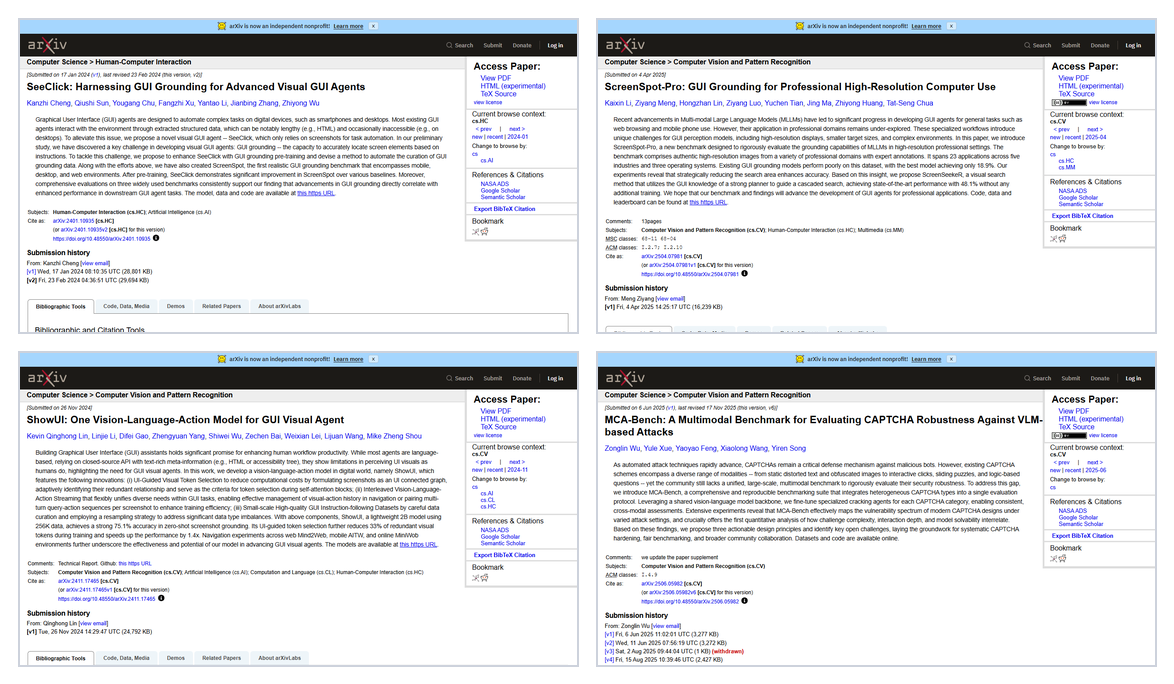
\includegraphics[width=0.96\linewidth]{related_work_web_montage.png}
  \caption{相关工作网页截图。图中展示 SeeClick、ScreenSpot-Pro、ShowUI 和 MCA-Bench 的论文页面，用于说明本项目调研了 GUI grounding、GUI action model 与多模态 CAPTCHA benchmark 三类相邻工作。}
  \label{fig:related-work-map}
\end{figure}

\section{数据集构造}

\subsection{合成图形九宫格数据}

项目首先实现了可程序生成的合成九宫格数据。每张图片被划分为九个格子，每个格子中绘制一个带颜色的对象。对象类别包括消防栓、汽车、自行车、路灯、树、信号灯、房子、星星和旗帜；颜色包括红色、蓝色、绿色、黄色、紫色、橙色、粉色、青色和黑色。每条样本同时保存图像路径、中文提示、目标格子编号和每格对象信息。

合成数据提供三种难度：
\begin{itemize}[leftmargin=2em]
  \item \textbf{easy：}九个格子的颜色唯一，指令包含颜色和物体类别，颜色基线即可完成大部分任务；
  \item \textbf{medium：}颜色可能重复，但物体类别唯一，模型需要同时利用颜色和形状信息；
  \item \textbf{hard：}指令只包含物体类别，颜色信息不可用，模型必须依赖视觉形状匹配。
\end{itemize}

\begin{figure}[H]
  \centering
  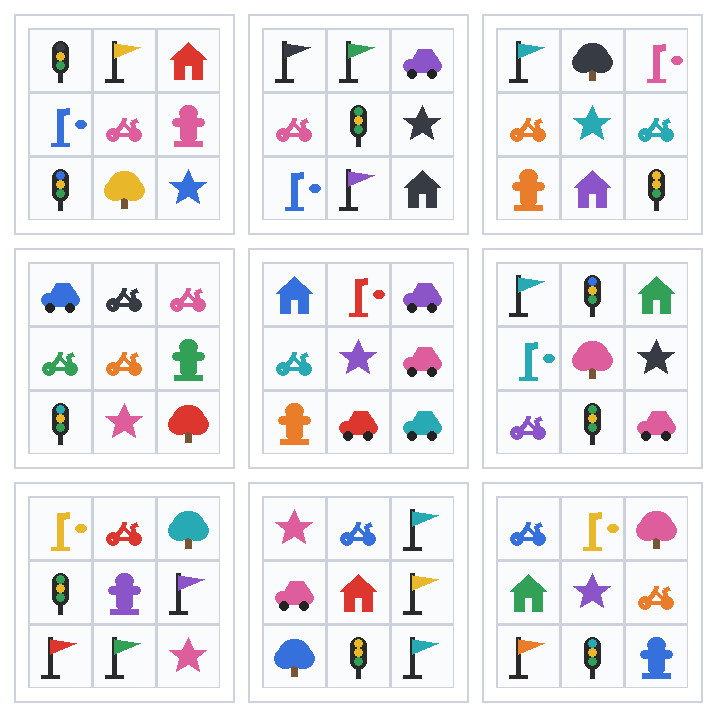
\includegraphics[width=0.72\linewidth]{dataset_synthetic_montage.png}
  \caption{合成九宫格样本拼图。合成数据用于 sanity check，帮助验证提示解析、格子编号、动作标签和评估脚本是否正确。}
  \label{fig:synthetic-sample}
\end{figure}

\subsection{真实照片九宫格数据}

为了缩小合成图形与真实图像之间的差距，项目进一步使用 Open Images 中的物体裁剪图片构造真实照片九宫格。每个类别的裁剪图片保存到 \pathcode{data/photo_objects/}，再由脚本拼接成九宫格样本。当前 100 类真实照片实验使用的数据目录为 \pathcode{data/photo_grid_100cls/}，总样本数为 10000 条。默认划分比例为 \code{train\_ratio=0.85}，即训练集 8500 条、验证集 1500 条。

真实照片数据构造时启用了 \code{--hard-augment}，对每个 cell 内图片进行随机裁剪、旋转、亮度与对比度变化、颜色扰动、模糊和噪声增强。该设置使训练样本更接近复杂网页场景中的视觉扰动，也能更好检验模型在细粒度类别上的鲁棒性。

\subsection{Click-all 动作序列数据}

在单目标定位基础上，项目进一步构造了“点击所有同类目标”的动作序列数据。每张九宫格中同一目标类别会出现 2 到 4 次，文本提示形如“请点击所有汽车”。标签不再是单个格子编号，而是目标格子集合 \code{target\_indices}，并可转换为动作序列：
\[
  [\text{move\_to\_cell}(i_1),\ \text{click},\ldots,\text{move\_to\_cell}(i_k),\ \text{click},\ \text{done}].
\]
该任务更接近真实网页交互，因为模型必须同时解决目标识别、目标数量判断、阈值选择和点击顺序生成。

为了减少数据泄露，我们在 click-all 数据构造器中加入 source-disjoint split：先按原始图片文件划分 train/val/test，再分别组合九宫格，避免同一来源图片同时出现在训练集和测试集。针对实验中发现的弱类，如裙子、帐篷、船、人、玩具，构造器进一步加入 source image quality filter，过滤原图面积过小、长宽比过极端、以及人工标注为明显坏源图的样本。最终的 paired dirty/clean 实验使用同一个 source pool 和 split plan，区别只在是否应用质量过滤和 blacklist，使数据清洗效果更可回溯。

\begin{figure}[H]
  \centering
  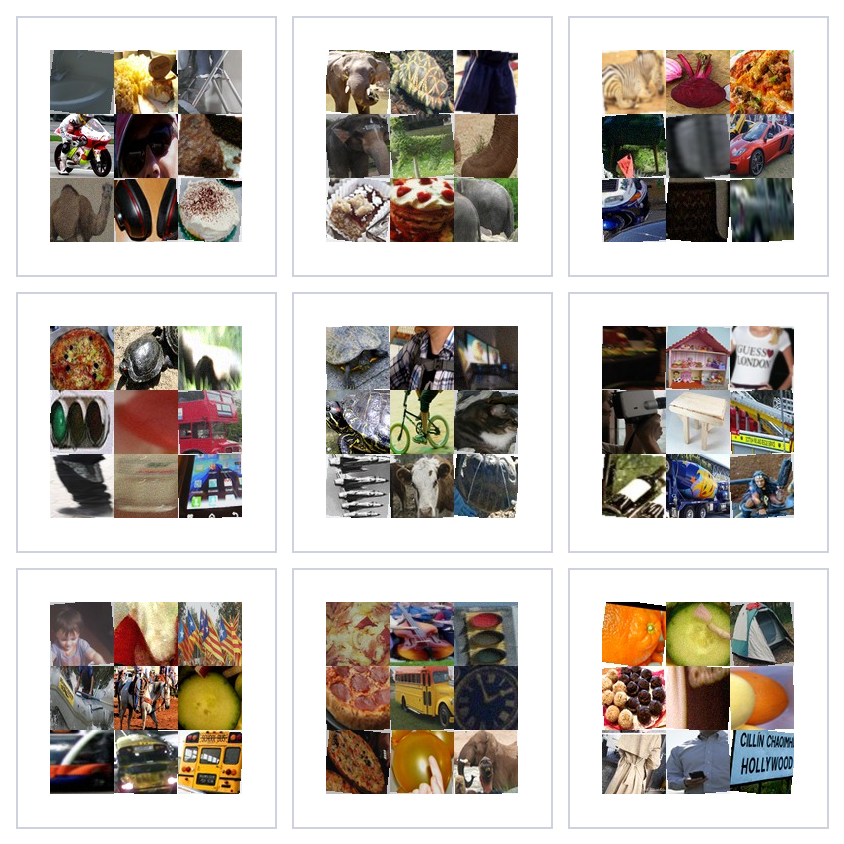
\includegraphics[width=0.84\linewidth]{dataset_photo_action_montage.png}
  \caption{真实照片 click-all 九宫格样本拼图。相比合成图形，真实照片包含裁剪不完整、背景复杂、目标尺度变化和弱类歧义等问题，因此更适合检验模型泛化能力。}
  \label{fig:data-pipeline}
\end{figure}

\begin{figure}[H]
  \centering
  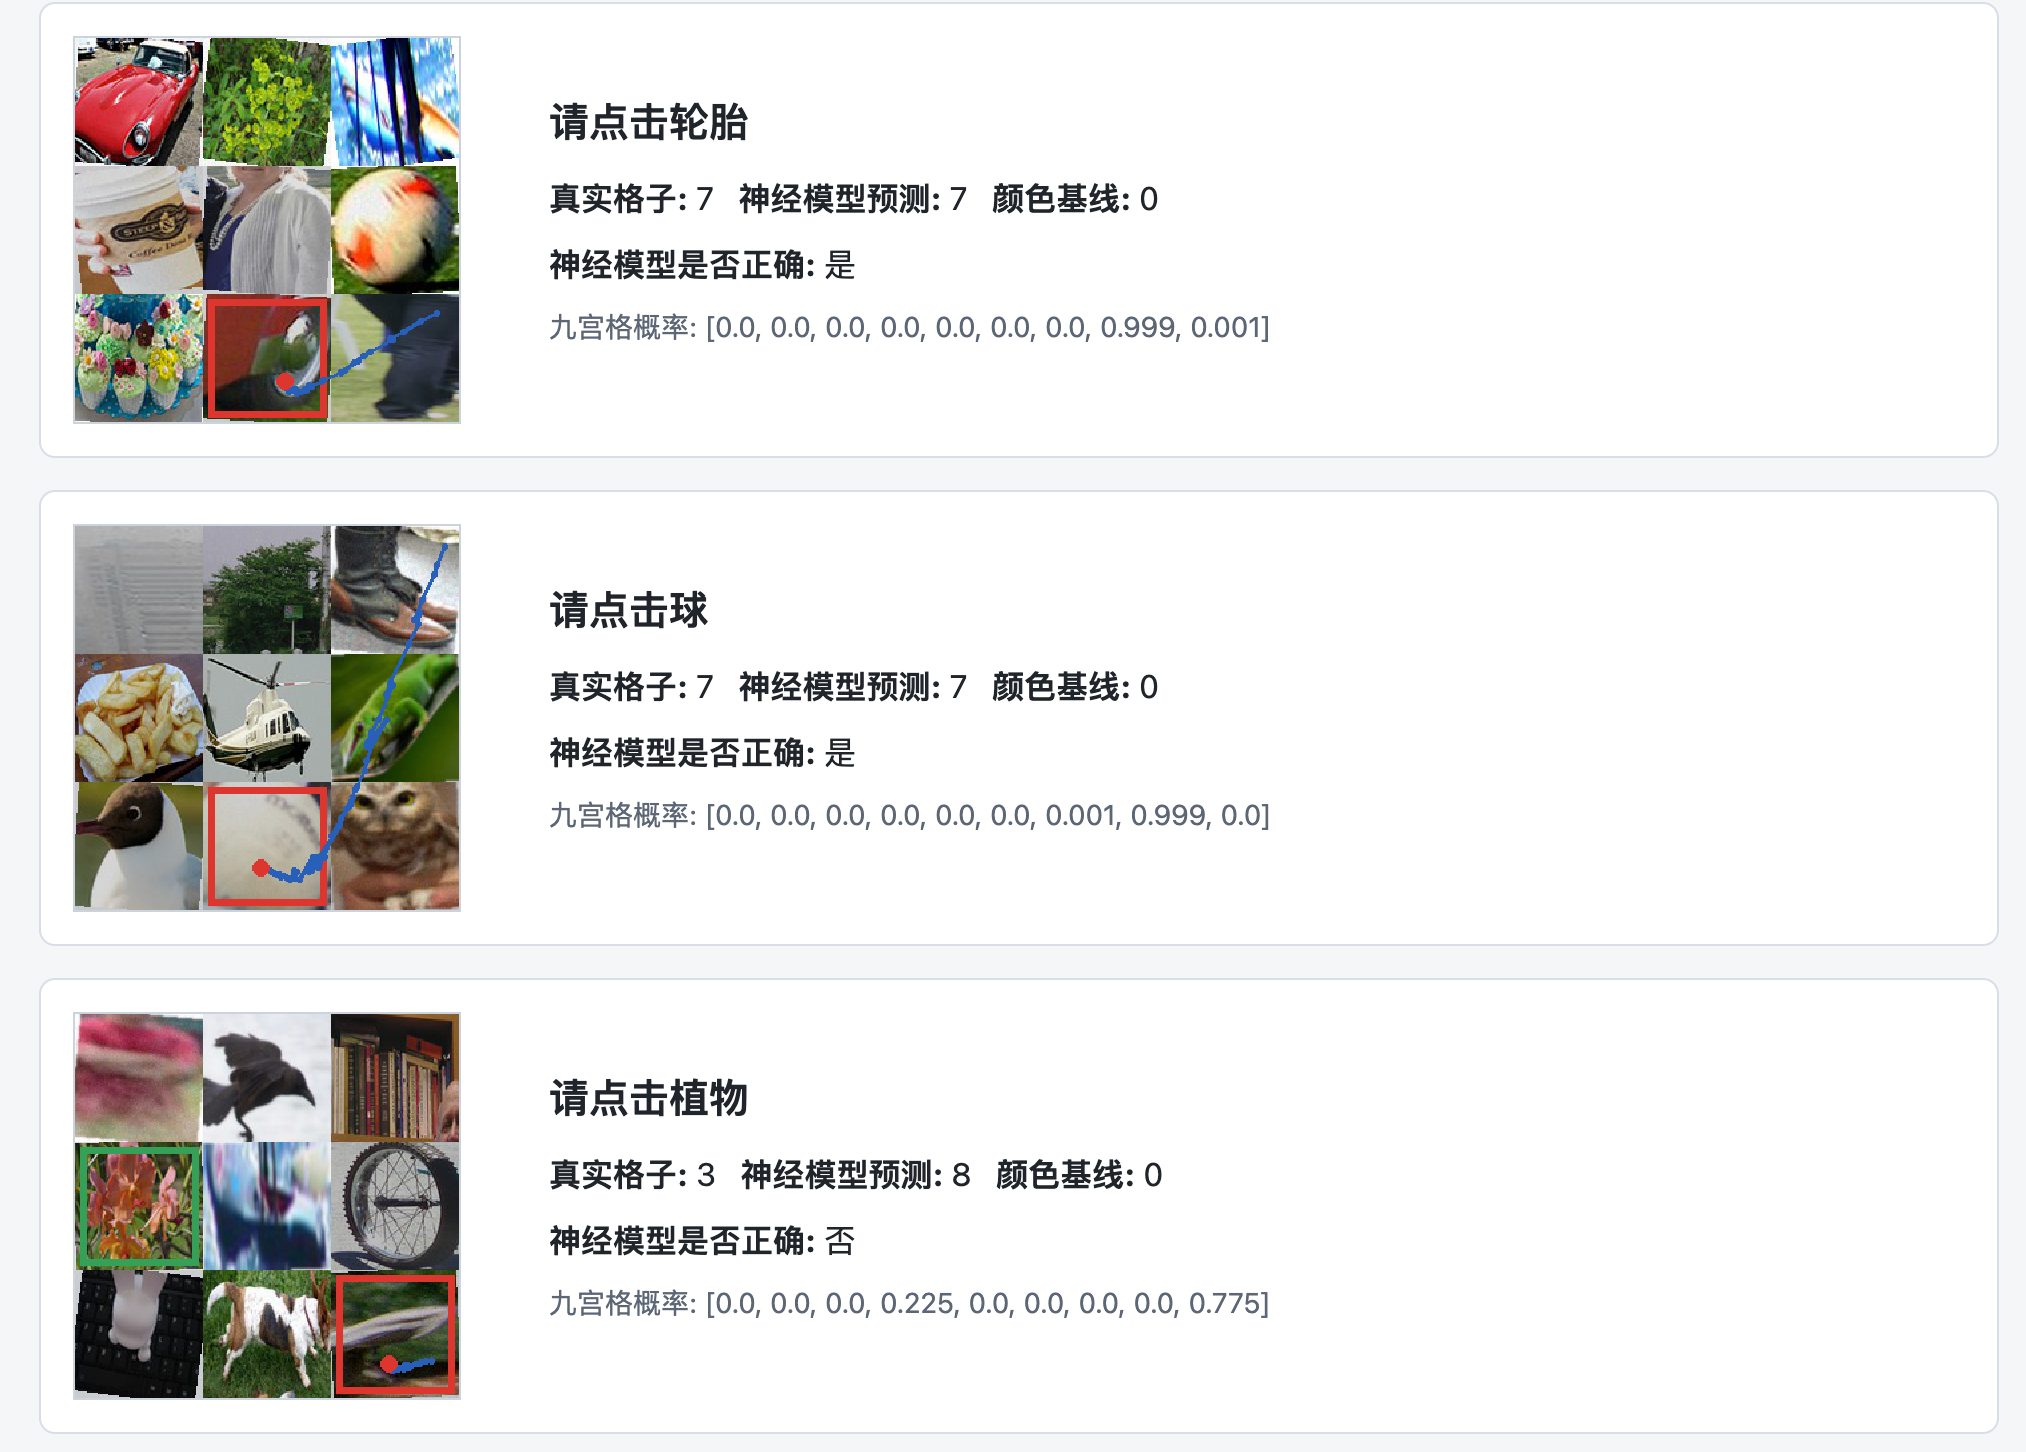
\includegraphics[width=0.68\linewidth]{single_target_demo.png}
  \caption{RoboTest 九宫格视觉定位示例。模型根据中文提示在九个候选格子中预测目标位置，并可视化预测结果。}
  \label{fig:demo}
\end{figure}

\section{算法设计思路}

\subsection{问题导向的迭代设计流程}

本项目的算法设计不是一次性确定的，而是在实验过程中围绕具体失败现象逐步迭代。整体思路可以概括为：
\begin{enumerate}[leftmargin=2em]
  \item \textbf{先建立可解释 sanity check：}使用规则颜色基线和模板匹配确认数据标签、格子编号和评估脚本正确；
  \item \textbf{再引入可训练模型：}当合成规则不足以覆盖真实照片时，加入 CNN、BiGRU 和 attention 融合模型；
  \item \textbf{再修正评估协议：}发现早期结果可能受样本级划分影响后，改造数据构建器支持 source-disjoint split；
  \item \textbf{再处理数据质量：}发现裙子、帐篷、船、人、玩具等弱类集中失败后，引入 source quality filter 和 blacklist；
  \item \textbf{再扩展动作任务：}单目标预测无法覆盖连续点击需求，因此扩展为 click-all 多标签选择和动作 token 输出；
  \item \textbf{最后补足自然提示：}模型对颜色、位置、功能性表达理解不足，因此增加 prompt rewrite、query planner 和属性 scorer。
\end{enumerate}

\begin{figure}[H]
  \centering
  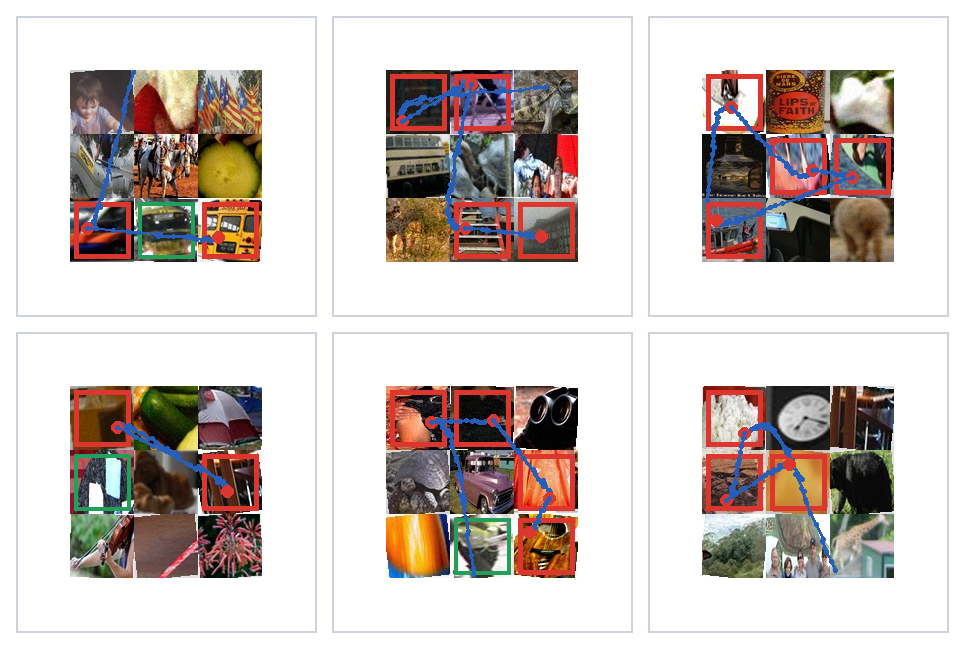
\includegraphics[width=0.84\linewidth]{failure_clean_montage.png}
  \caption{问题导向设计的依据：专训模型在 clean paired 测试集上的失败样例。失败图直接暴露出漏点、多点、目标过小和类别边界不清等问题，推动了数据清洗、弱类 blacklist 和阈值校准。}
  \label{fig:design-iteration}
\end{figure}

\subsection{总体流程}

RoboTest 的整体流程包括四个阶段：数据生成、图文定位、点击点预测和轨迹生成。首先，系统生成或读取九宫格图像，并为每条样本保存文本指令和目标格子标签；其次，定位模型根据图像和文本预测九个格子的匹配分数；然后，系统将最高分格子转换为点击坐标；最后，轨迹模块从随机起点到目标点生成带曲线、速度变化、抖动和末端停顿的鼠标移动轨迹。

\begin{figure}[H]
  \centering
  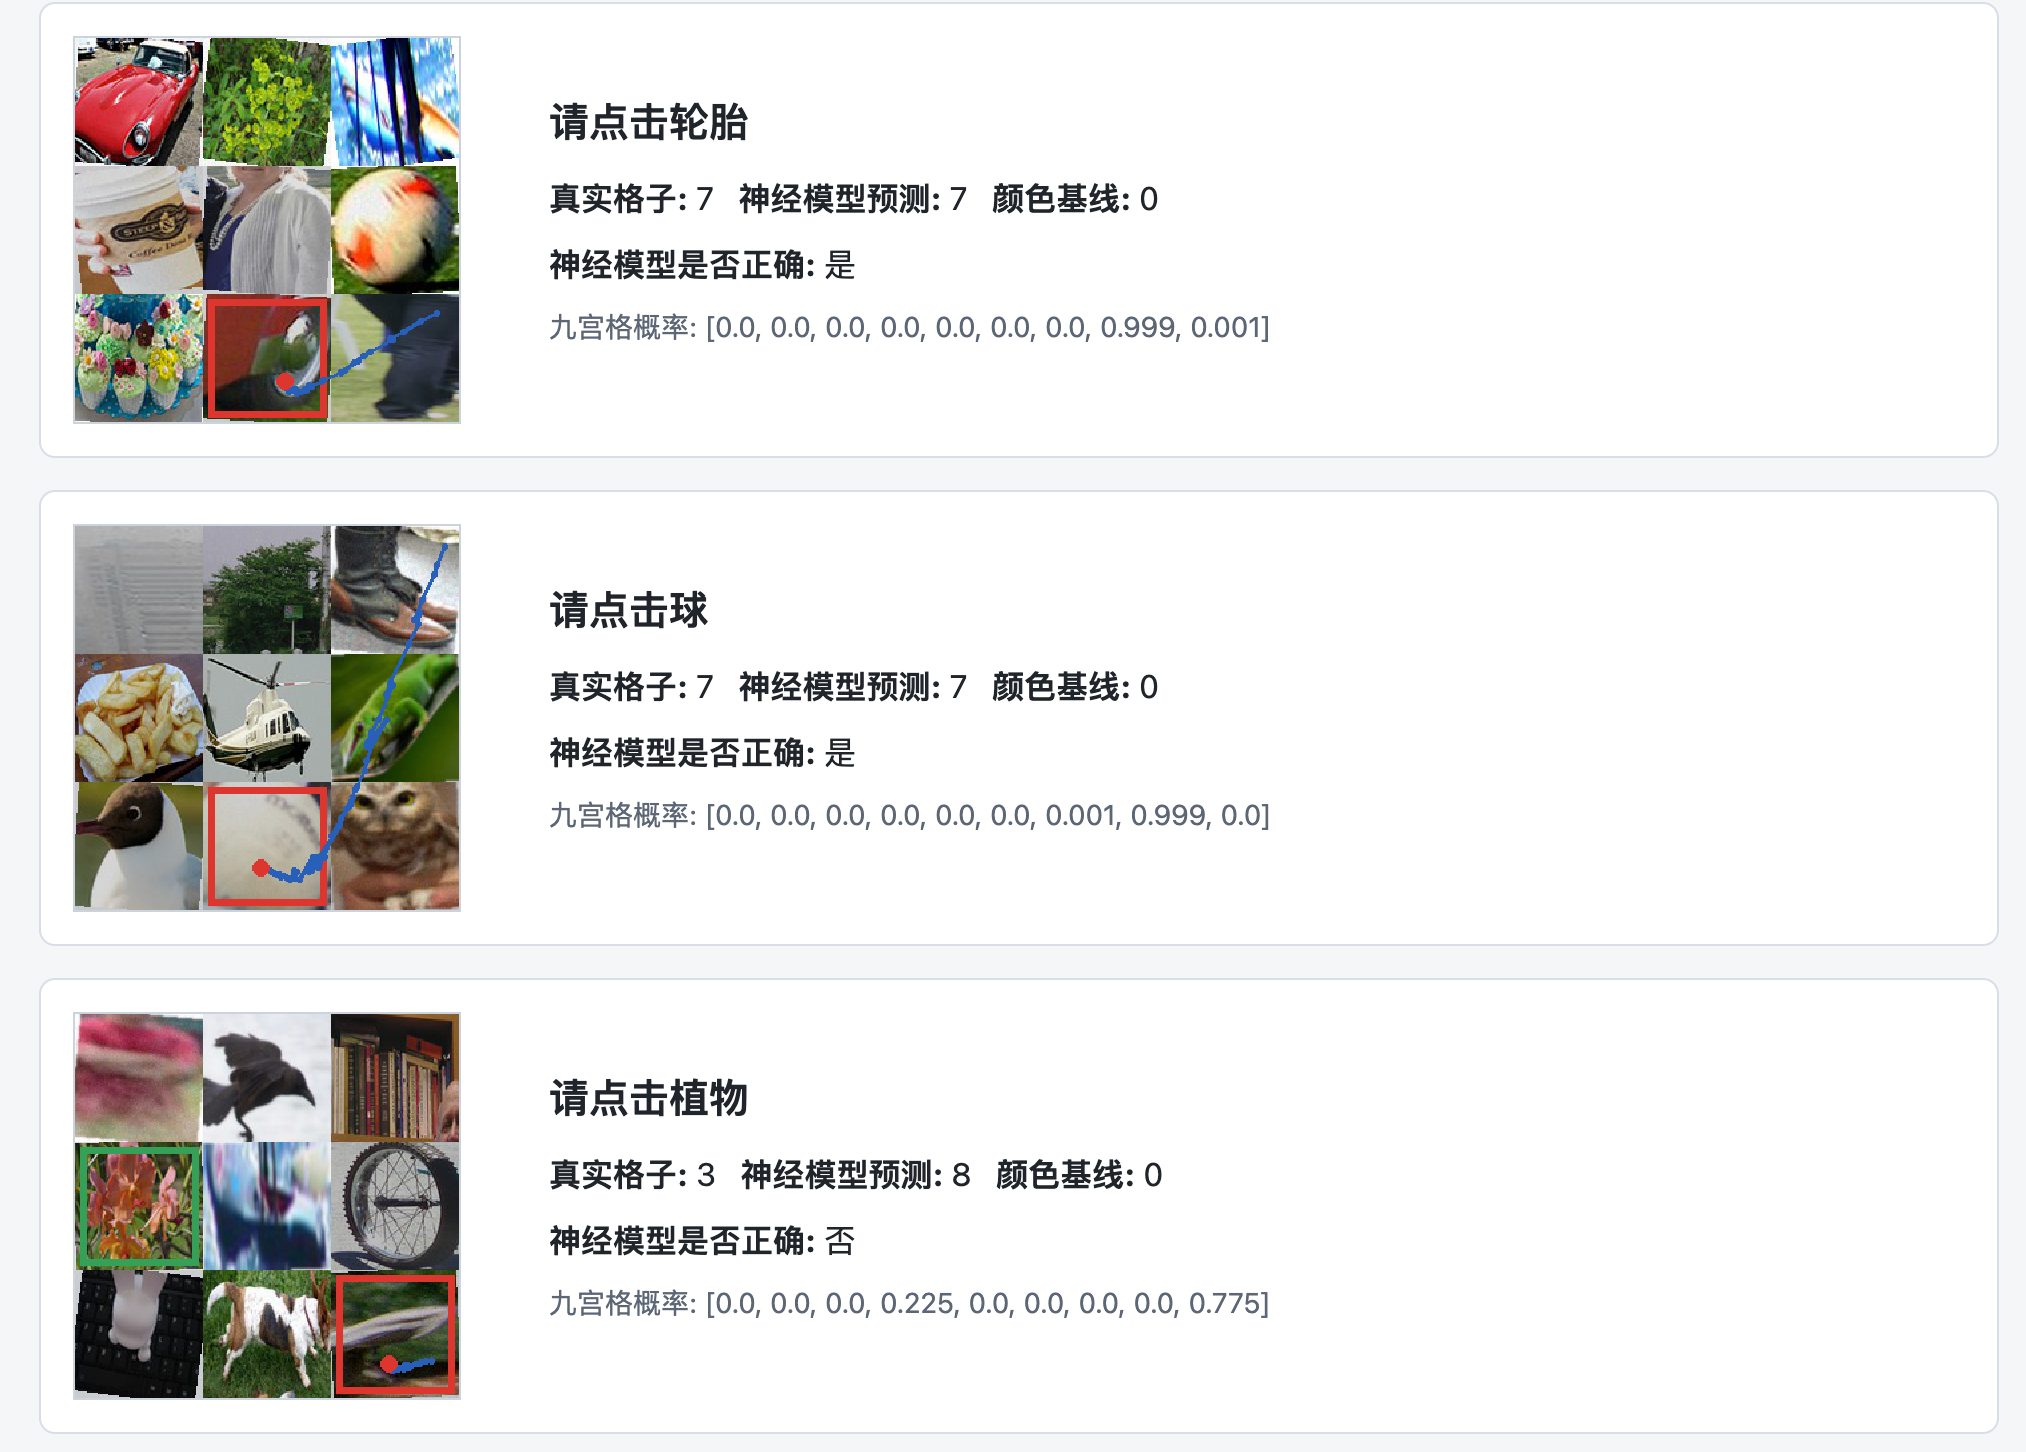
\includegraphics[width=0.68\linewidth]{single_target_demo.png}
  \caption{单目标定位模型的真实可视化输出。模型以九宫格图片和中文提示为输入，输出目标格概率、预测点击点和模拟鼠标轨迹。}
  \label{fig:single-target-output}
\end{figure}

\subsection{规则颜色基线}

规则颜色基线用于建立一个简单、可解释的对照方法。该方法从中文指令中解析目标颜色，然后对每个格子计算像素颜色匹配分数，选择颜色最接近的格子作为预测结果。在 easy 数据中，颜色唯一且指令包含颜色，因此该基线能取得很高准确率；但在 medium 难度中颜色会重复，在 hard 难度中文本不再提供颜色，因此该方法会明显退化。

\subsection{模板图文匹配模型}

模板图文匹配模型在规则颜色基础上加入物体形状信息。它先从中文指令中解析颜色和物体类别，再为目标类别生成形状模板；图像侧对每个格子提取颜色匹配分数和前景形状相似度，最后融合两类分数得到九个格子的概率分布。该方法不需要训练，适合合成图形数据，并能清楚展示“文本条件 + 视觉特征”的匹配过程。

\subsection{注意力增强神经模型}

真实照片九宫格任务中，模板匹配难以泛化到复杂纹理、背景和裁剪变化，因此项目实现了可训练的多模态定位模型 \code{MultimodalGridLocator}。该模型包含文本分支、图像分支、九格上下文建模和图文融合四个部分。

文本分支采用字符级 tokenization，将中文指令输入 Embedding 层，再经过双向 GRU 得到文本特征 $f_t$。字符级建模虽然简单，但对“请点击汽车”“请点击披萨”等短中文指令足够稳定，也降低了额外中文分词依赖。

图像分支先将整张九宫格切分为 9 个 cell，并将每个 cell resize 到 $96\times96$。每个 cell 经过残差 CNN 提取局部视觉特征，再通过线性层投影到统一维度。注意力增强版本在九个 cell 特征上加入位置编码，并使用 2 层 Transformer Encoder 建模格子之间的上下文关系。

图文融合阶段，对每个格子拼接四类特征：
\[
  z_i = [f_i,\ f_t,\ f_i \odot f_t,\ |f_i-f_t|],
\]
其中 $f_i$ 表示第 $i$ 个格子的视觉特征，$f_t$ 表示文本特征，$\odot$ 表示逐维乘积。拼接后的特征输入 MLP，输出每个格子的 logit。最终使用 softmax 得到概率分布，并取最大概率格子作为预测结果。

\subsection{损失函数与辅助监督}

训练时主任务是九分类定位，使用 CrossEntropyLoss 约束目标格子预测。为了让图像编码器更明确地学习每个格子中的物体类别，模型额外加入 \code{object\_head} 辅助分类头，对每个 cell 预测物体类别。总损失定义为：
\[
  \mathcal{L} = \mathcal{L}_{grid} + \lambda \mathcal{L}_{object},
\]
其中 $\lambda$ 为辅助损失权重，当前实验中设置为 0.7。该设计的动机是将“找目标格子”的弱监督问题拆解出“识别每格物体”的辅助目标，从而提升真实照片场景下的视觉特征质量。

\subsection{鼠标轨迹生成}

定位模型输出目标格子后，轨迹模块根据目标格子的几何位置生成点击轨迹。早期版本使用固定左上角起点和格子中心终点，当前版本改为随机边缘或图内起点、目标格内部随机落点，并加入曲线插值、速度变化、轻微抖动和末端停顿。该模块使系统输出不只包含分类结果，还能形成一个完整的点击交互流程。

\subsection{Click-all Action Sequence 模型}

Click-all 模型将九宫格定位从单标签分类扩展为多标签 cell selection。图像侧仍按九个 cell 提取视觉特征，文本侧编码“请点击所有某类别”的中文指令，融合后对每个 cell 输出一个独立概率。推理时，模型根据阈值选择所有目标格；如果没有 cell 超过阈值，则回退到 top-1，避免输出空动作。被选中的 cell 按从小到大的格子编号转换为动作序列，形成可执行的 \code{move\_to\_cell/click/done} 输出。最终模型的完整数据流如图~\ref{fig:model-architecture} 所示。

阈值选择是该任务的关键。过低阈值会提升 recall 但引入多余点击，过高阈值会提升 precision 但漏点目标。项目最初从 0.1 开始搜索阈值，后来在失败分析中发现部分目标概率整体偏低，因此将默认 grid 扩展为 \code{0.03, 0.05, 0.07, 0.1, ...}。最终评估脚本支持 \code{--threshold auto}，在验证集上选择阈值，再固定到测试集，避免直接在测试集上调参。

\begin{figure}[H]
  \centering
  \resizebox{\linewidth}{!}{%
  \begin{tikzpicture}[
    font=\sffamily\small,
    node distance=6mm and 8mm,
    box/.style={draw=black!55, line width=0.55pt, rounded corners=2pt, align=center, minimum height=12mm, text width=25mm, inner sep=4pt},
    input/.style={box, fill=archinput},
    textbranch/.style={box, fill=archtext},
    visionbranch/.style={box, fill=archvision},
    fusion/.style={box, fill=archfusion, text width=32mm},
    output/.style={box, fill=archoutput},
    aux/.style={box, fill=archaux, text width=27mm},
    flow/.style={-{Stealth[length=2.2mm]}, line width=0.8pt, draw=black!70},
    optional/.style={-{Stealth[length=2.2mm]}, line width=0.7pt, dashed, draw=black!55}
  ]
    \node[input] (prompt) {中文指令\\``请点击所有汽车''};
    \node[textbranch, right=of prompt] (textenc) {字符 Token\\Embedding + BiGRU\\文本特征 $f_t$};

    \node[input, below=9mm of prompt] (image) {$3\times3$ 九宫格图像 $I$};
    \node[visionbranch, right=of image] (vision) {切分 9 个 cell\\Resize $96\times96$\\共享 ResNet18};
    \node[visionbranch, right=of vision] (cellfeat) {线性投影 + 位置编码\\cell 特征 $f_i$};

    \node[fusion, right=10mm of cellfeat, yshift=10mm] (fusion) {九格图文交互\\$[f_i; f_t; f_i\odot f_t; |f_i-f_t|]$};
    \node[output, right=of fusion] (selector) {MLP Cell Selector\\9 个独立 logits};
    \node[output, right=of selector] (decode) {Sigmoid + 自动阈值\\无命中时 top-1};
    \node[output, right=of decode] (selected) {目标格集合\\$\{c_1,\ldots,c_k\}$};
    \node[output, right=of selected] (actions) {动作序列\\move / click / done};
    \node[output, right=of actions] (trajectory) {格内落点\\平滑鼠标轨迹};

    \node[aux, below=8mm of fusion] (objecthead) {辅助 Object Head\\每格类别监督\\仅训练阶段};
    \node[aux, below=8mm of selector] (counthead) {可选 Count Head\\$\mathrm{mean}(f_i)\oplus f_t\rightarrow k$\\top-k 解码};

    \draw[flow] (prompt) -- (textenc);
    \draw[flow] (image) -- (vision);
    \draw[flow] (vision) -- (cellfeat);
    \draw[flow] (textenc.east) -| (fusion.north west);
    \draw[flow] (cellfeat.east) -| (fusion.south west);
    \draw[flow] (fusion) -- (selector);
    \draw[flow] (selector) -- (decode);
    \draw[flow] (decode) -- (selected);
    \draw[flow] (selected) -- (actions);
    \draw[flow] (actions) -- (trajectory);
    \draw[optional] (cellfeat.south east) |- (objecthead.west);
    \draw[optional] (fusion.south) -- (counthead.west);
    \draw[optional] (counthead.east) -| (selected.south);

  \end{tikzpicture}%
  }
  \caption{RoboTest 最终 click-all 多模态模型架构。主路径将中文指令与九格视觉特征交互融合，独立预测每格点击分数，再解码为动作序列和鼠标轨迹；虚线为 object 辅助监督和可选 count-head top-k 路径。}
  \label{fig:model-architecture}
\end{figure}

\begin{figure}[H]
  \centering
  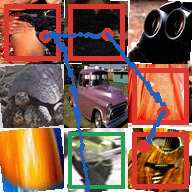
\includegraphics[width=0.62\linewidth]{click_all_failure_example.png}
  \caption{Click-all 动作序列任务示例。图中红框与绿框展示预测集合和真实集合的差异，体现该任务不仅要识别类别，还要判断目标数量并控制点击集合。}
  \label{fig:action-sequence-flow}
\end{figure}

\subsection{提示词改写与属性执行器}

实际用户提示并不总是直接落在训练类别上。例如“请点击可以演奏音乐的物体”需要映射到吉他、大提琴等已有类别；“请点击红色物体”只给出颜色属性，而我们的主模型主要学习物体类别。为此，Web demo 中加入了两层补救机制：第一，使用 DeepSeek 文本模型或规则 fallback 将抽象提示改写为训练类别提示；第二，使用 query planner 将提示解析为 \code{object\_only}、\code{color\_only}、\code{object\_plus\_attributes}、\code{position\_only} 等结构，再调用颜色、位置、大小等轻量属性 scorer 执行。这部分不替代主模型训练，但可以提高演示系统对真实用户表达方式的容错能力。

\begin{figure}[H]
  \centering
  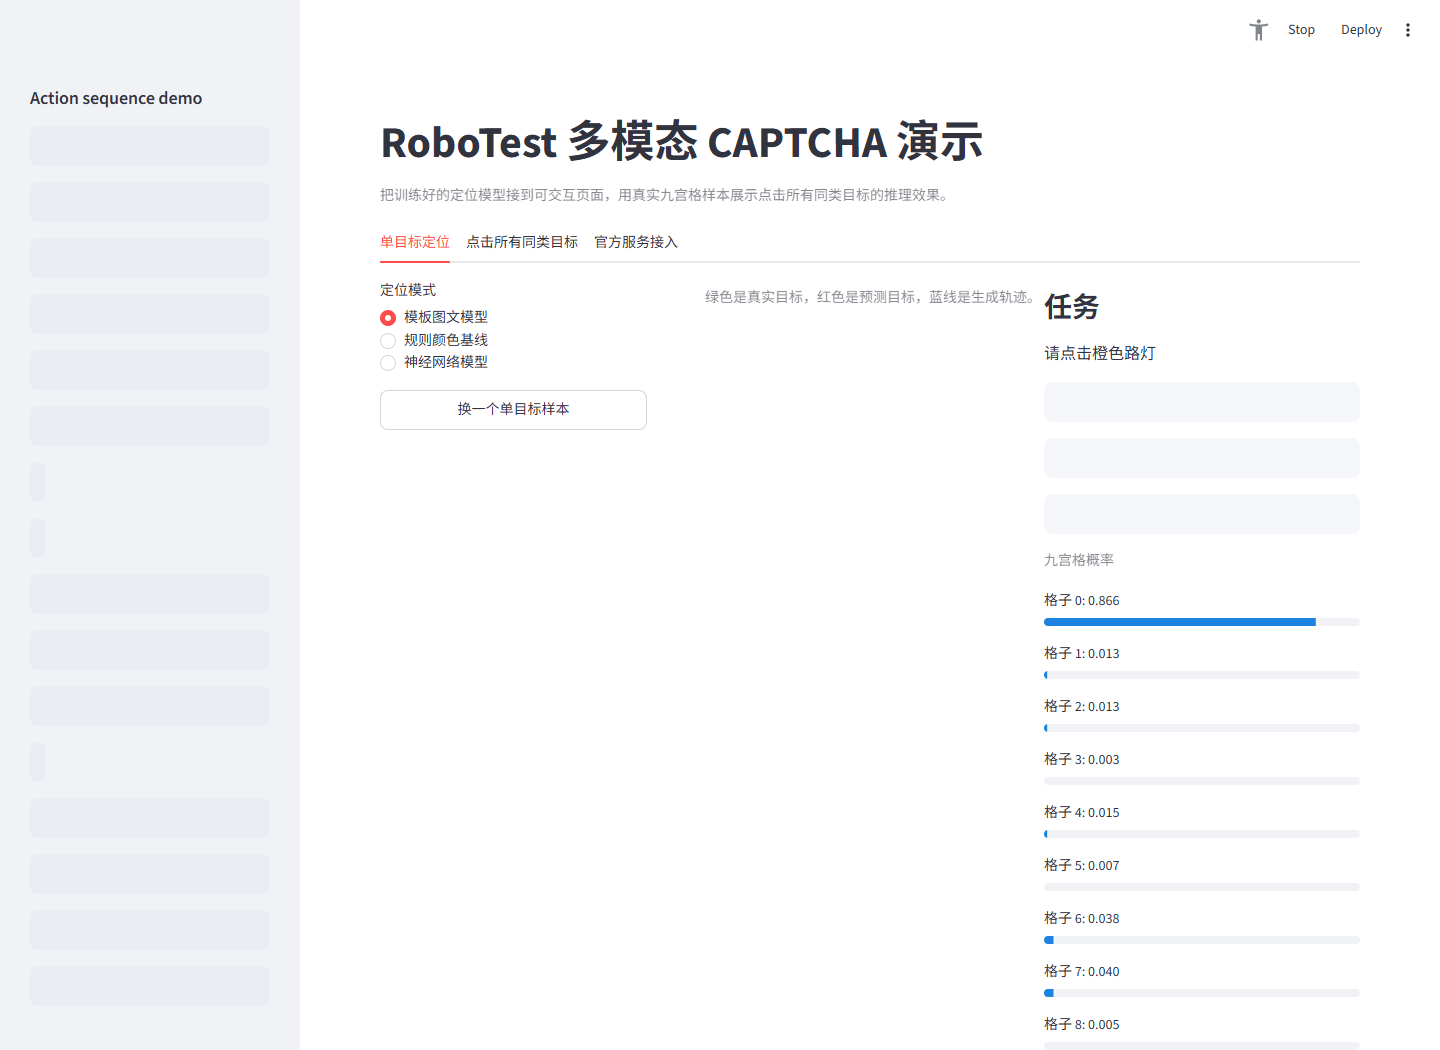
\includegraphics[width=0.96\linewidth]{streamlit_demo.png}
  \caption{提示词处理与模型推理的 Web 展示截图。页面提供手动 prompt、单目标定位、click-all 推理、提示词改写和 VLM 对比入口，方便观察自然语言输入如何影响模型输出。}
  \label{fig:prompt-planner-flow}
\end{figure}

\section{实验设置}

\subsection{训练参数}

100 类真实照片 attention 模型的训练命令如下：

\begin{verbatim}
python scripts/train.py \
  --data-dir data/photo_grid_100cls \
  --output outputs/photo_model_100cls_attn.pt \
  --epochs 40 \
  --batch-size 64 \
  --lr 0.001 \
  --aux-weight 0.7 \
  --patience 10 \
  --model-size attn \
  --progress-every 20
\end{verbatim}

训练使用 AdamW 优化器和 CosineAnnealingLR 学习率调度器。训练日志以 JSONL 格式保存，记录 batch 进度、loss、ETA、每轮验证准确率和最佳验证准确率。模型权重保存到 \code{outputs/photo\_model\_100cls\_attn.pt}。

\begin{table}[H]
  \centering
  \caption{100 类真实照片九宫格实验配置。}
  \label{tab:config}
  \begin{tabular}{ll}
    \toprule
    \rowcolor{tablehead}
    配置项 & 取值 \\
    \midrule
    数据目录 & \code{data/photo\_grid\_100cls/} \\
    样本数 & 10000 \\
    训练/验证划分 & 8500 / 1500 \\
    模型 & \code{MultimodalGridLocator}, \code{model-size=attn} \\
    文本编码器 & 字符 Embedding + 双向 GRU \\
    图像编码器 & 残差 CNN，每格 resize 到 $96\times96$ \\
    上下文建模 & 2 层 Transformer Encoder \\
    batch size & 64 \\
    epochs & 40 \\
    learning rate & 0.001 \\
    auxiliary weight & 0.7 \\
    optimizer & AdamW \\
    scheduler & CosineAnnealingLR \\
    \bottomrule
  \end{tabular}
\end{table}

\subsection{评价指标}

本项目主要使用以下指标评价模型效果：
\begin{itemize}[leftmargin=2em]
  \item \textbf{Grid Accuracy：}预测格子编号是否与真实目标格一致；
  \item \textbf{Top-3 Accuracy：}真实目标是否出现在概率最高的 3 个格子中；
  \item \textbf{Mean Click Distance：}预测点击点与真实点击点之间的平均距离；
  \item \textbf{Median Click Distance：}点击距离中位数；
  \item \textbf{Failure Cases：}保存失败样例图，便于进行定性分析。
\end{itemize}

对于 click-all action sequence 任务，单个样本可能包含多个目标格，因此额外使用以下指标：
\begin{itemize}[leftmargin=2em]
  \item \textbf{Cell Exact Match：}预测目标格集合是否与真实集合完全一致；
  \item \textbf{Cell Precision：}预测点击的格子中有多少是真实目标；
  \item \textbf{Cell Recall：}真实目标格中有多少被成功点击；
  \item \textbf{Click Order Accuracy：}动作序列对应的点击顺序是否与标准顺序一致；
  \item \textbf{Count Accuracy：}预测点击数量是否等于真实目标数量，主要用于 VLM baseline 分析。
\end{itemize}

\section{实验结果}

\subsection{合成图形数据结果}

合成数据实验用于验证不同难度下颜色、形状和图文匹配信息的重要性。表~\ref{tab:synthetic} 显示，规则颜色基线在 easy 难度中可以达到 1.000 accuracy，但在 medium 和 hard 难度中明显下降；模板图文匹配模型由于加入了物体形状模板，在合成 medium 和 hard 数据上仍能稳定完成任务。

\begin{table}[H]
  \centering
  \caption{合成图形九宫格数据上的方法对比。}
  \label{tab:synthetic}
  \begin{tabular}{llccc}
    \toprule
    \rowcolor{tablehead}
    数据设置 & 方法 & Accuracy $\uparrow$ & Top-3 $\uparrow$ & Mean Dist. $\downarrow$ \\
    \midrule
    easy & 规则颜色基线 & 1.000 & 1.000 & 0.000 \\
    easy & 模板图文匹配 & 1.000 & 1.000 & 0.000 \\
    medium & 规则颜色基线 & 0.333 & 1.000 & 70.960 \\
    medium & 模板图文匹配 & 1.000 & 1.000 & 0.000 \\
    hard & 规则颜色基线 & 0.111 & 0.333 & 108.423 \\
    hard & 模板图文匹配 & 1.000 & 1.000 & 0.000 \\
    默认 medium 600 & 规则颜色基线 & 0.433 & 1.000 & 56.632 \\
    默认 medium 600 & 模板图文匹配 & 1.000 & 1.000 & 0.000 \\
    \bottomrule
  \end{tabular}
\end{table}

\subsection{真实照片九宫格结果}

真实照片实验用于检验模型在更复杂视觉输入上的泛化能力。表~\ref{tab:photo} 总结了已有实验结果。对象感知 CNN 在 500 样本真实照片九宫格上取得 0.773 accuracy；进一步扩展到 100 类真实照片并使用 attention 模型后，Top-1 accuracy 达到 82.4\%，Top-3 accuracy 达到 96.87\%，平均点击距离为 28.64。

\begin{table}[H]
  \centering
  \caption{真实照片九宫格数据上的实验结果。}
  \label{tab:photo}
  \scriptsize
  \begin{tabular}{p{0.34\linewidth}p{0.13\linewidth}p{0.10\linewidth}p{0.13\linewidth}p{0.16\linewidth}}
    \toprule
    \rowcolor{tablehead}
    设置 & Acc./Top-1 $\uparrow$ & Top-3 $\uparrow$ & Mean Dist. $\downarrow$ & 说明 \\
    \midrule
    真实照片 500 样本，对象感知 CNN & 0.773 & 0.960 & 32.248 & 早期真实照片实验 \\
    真实照片 500 样本，残差 CNN 短训 & 0.333 & 0.680 & 108.796 & 训练轮数不足 \\
    100 类真实照片，attention 模型 & 0.824 & 0.9687 & 28.64 & 1500 条验证集 \\
    30k hard-negative，small 模型 & 0.9169 & -- & -- & 50 epochs 训练日志 \\
    \bottomrule
  \end{tabular}
\end{table}

\begin{figure}[H]
  \centering
  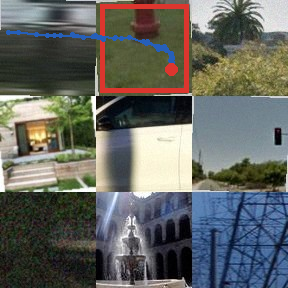
\includegraphics[width=0.72\linewidth]{hard_negative_prediction.png}
  \caption{相似类别 hard-negative 预测样例。该类样本把视觉上接近的类别放入同一九宫格，迫使模型学习更细粒度的区分能力。}
  \label{fig:hard-negative}
\end{figure}

\subsection{ResNet18 编码器训练方式消融}

为分析 click-all 模型的主要瓶颈，我们在 clean80 数据上对比了三种 ResNet18 编码器训练方式：参数冻结但保留历史 BatchNorm 统计量更新、仅训练最后一个 ResNet block，以及完整微调图像编码器。三组实验均使用 base action head、10000 条训练样本、2000 条验证样本、batch size 32 和 $3\times10^{-4}$ 学习率。

\begin{figure}[H]
  \centering
  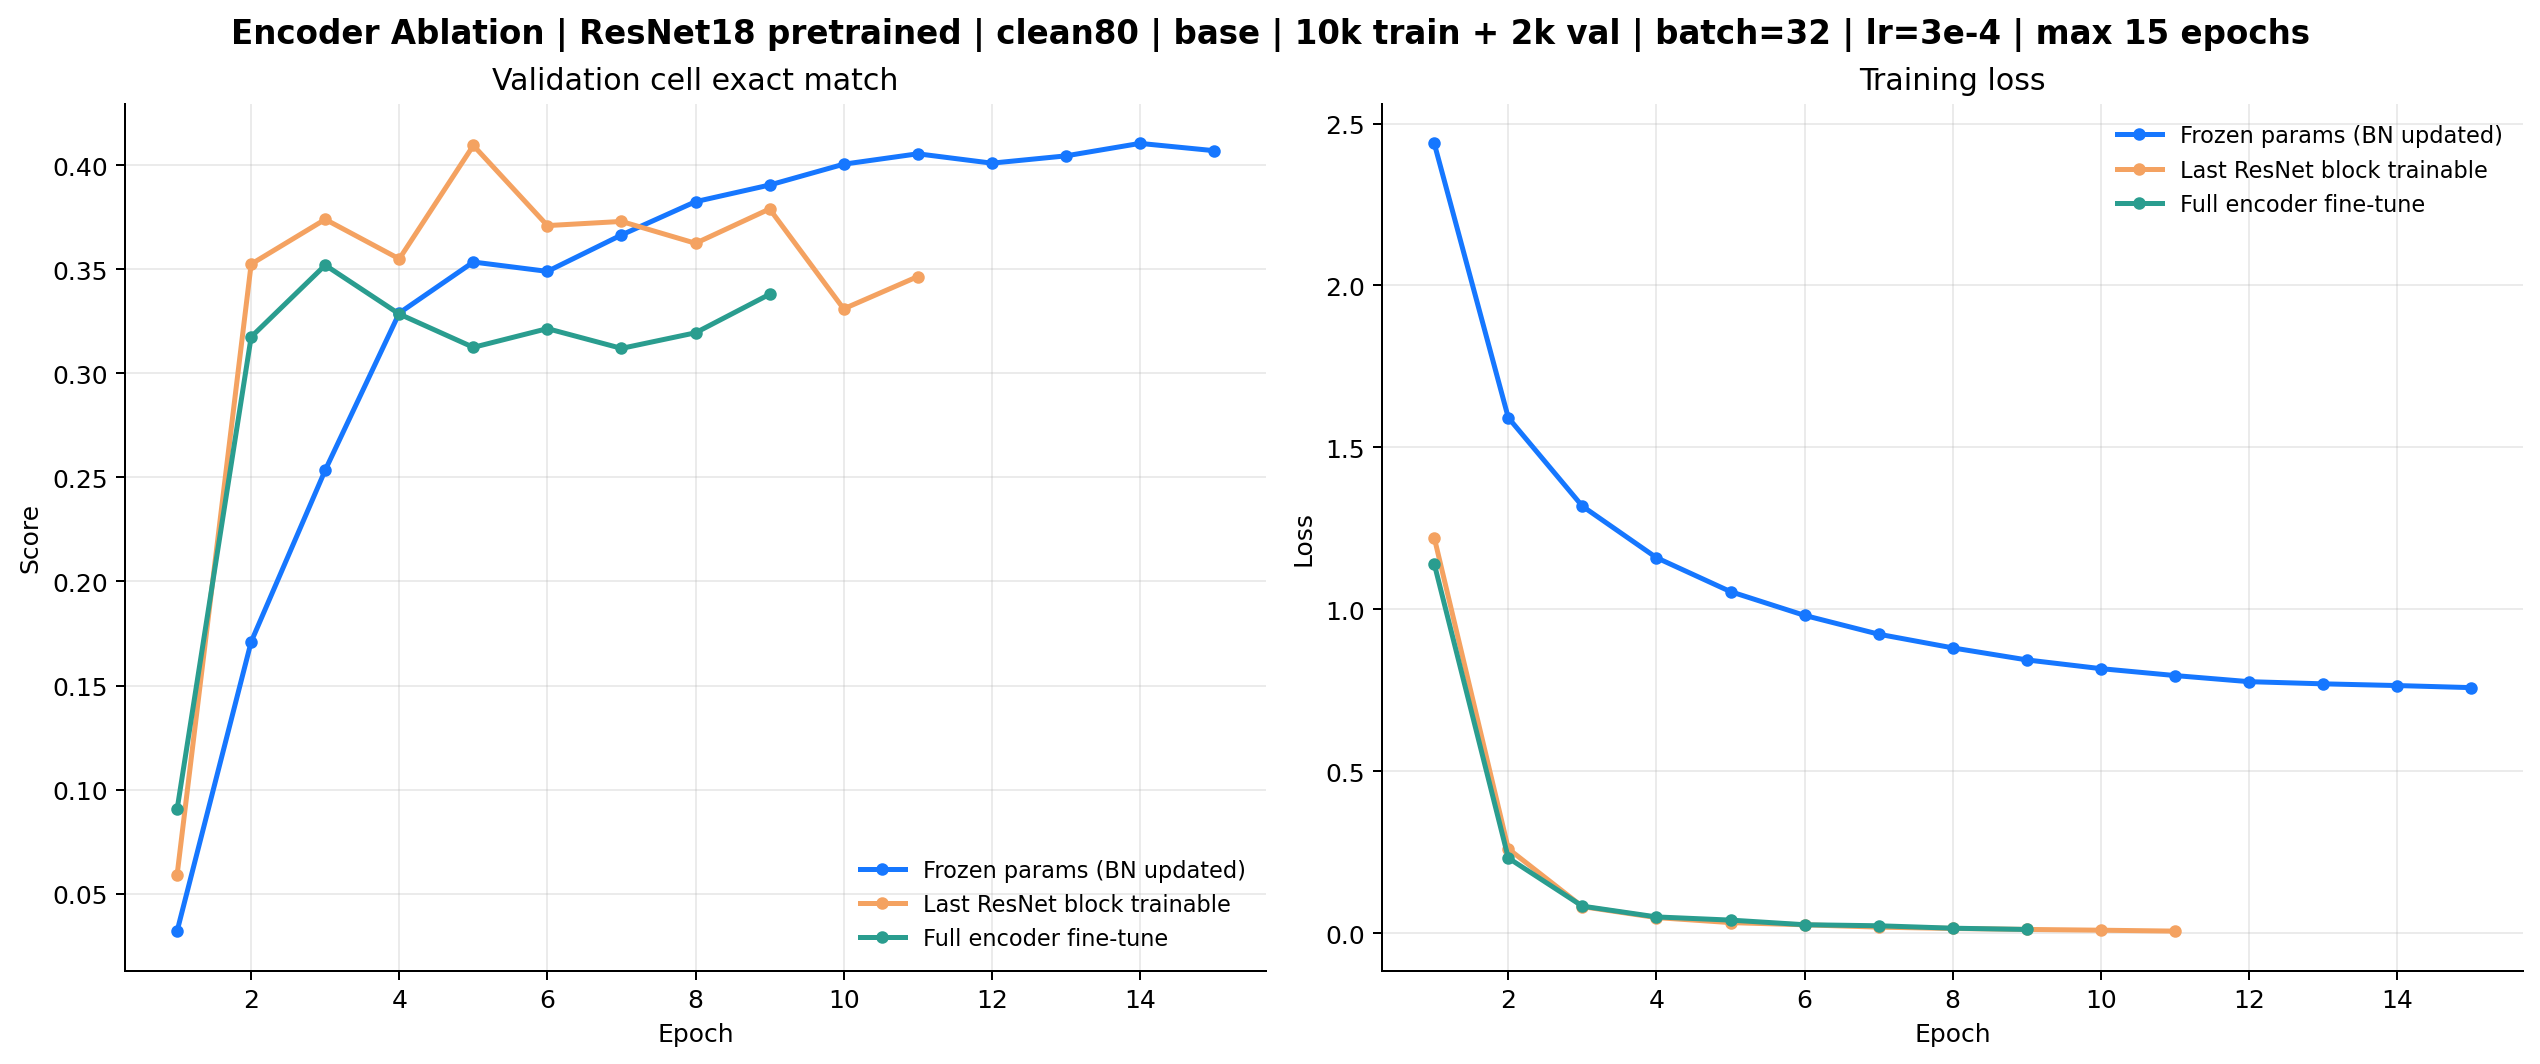
\includegraphics[width=0.96\linewidth]{resnet18_encoder_ablation.png}
  \caption{ResNet18 编码器训练方式消融。左图为验证集 cell exact match，右图为训练损失。部分微调与全量微调虽然快速将训练损失降至接近零，验证 exact match 却在较低水平波动；参数冻结设置收敛较慢，后期验证结果更稳定。}
  \label{fig:resnet18-encoder-ablation}
\end{figure}

\begin{figure}[H]
  \centering
  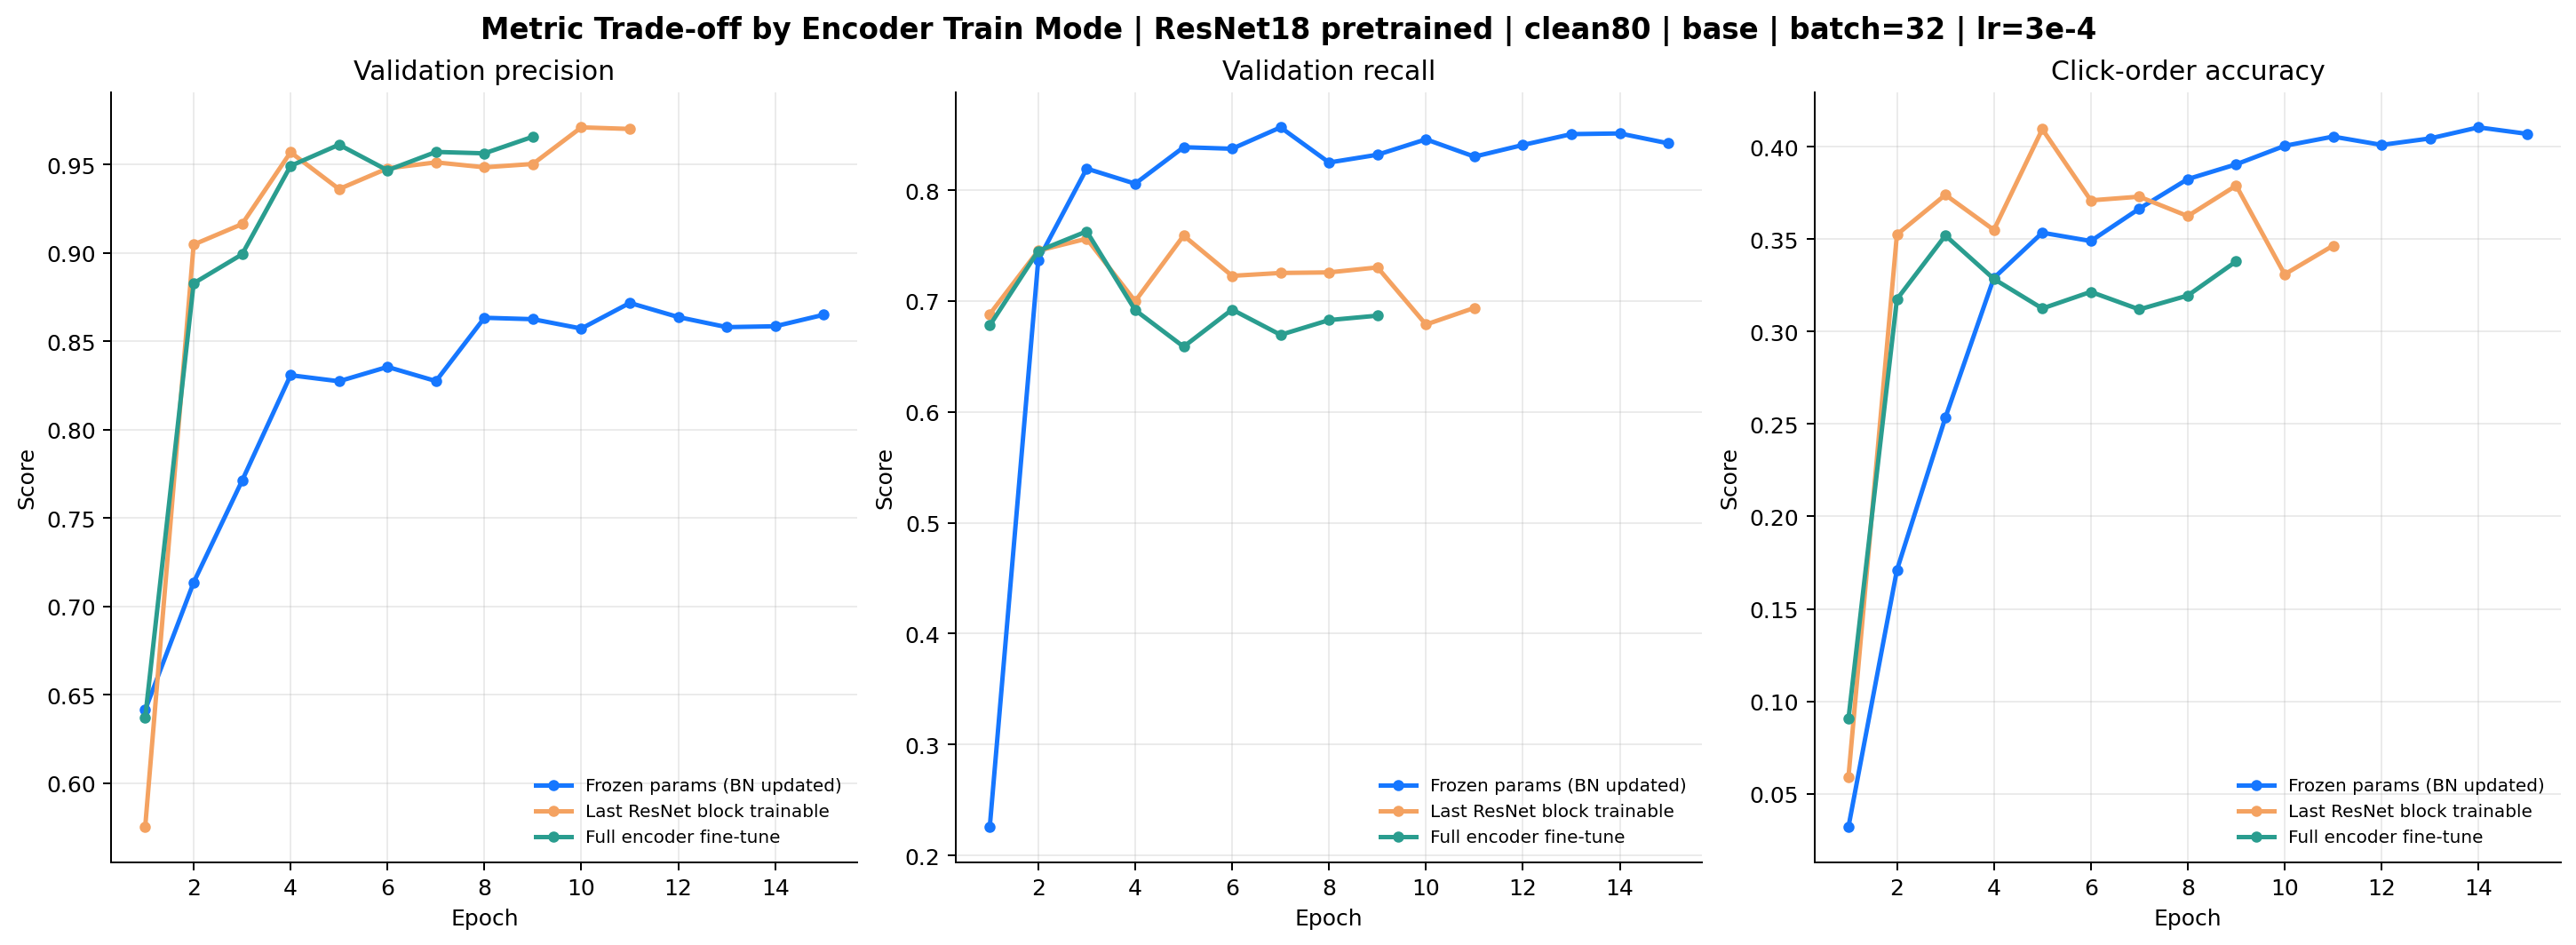
\includegraphics[width=0.96\linewidth]{resnet18_metric_tradeoff.png}
  \caption{ResNet18 编码器训练方式的验证指标权衡。部分微调和全量微调取得更高 precision，但 recall 和 click-order accuracy 较低；参数冻结设置在后期获得更均衡的召回率与动作序列准确率。}
  \label{fig:resnet18-metric-tradeoff}
\end{figure}

这组消融说明，训练损失更低并不必然意味着 click-all 集合预测更准确。在当前数据规模下，解冻较多视觉参数会更快拟合训练集，并倾向以更少的点击换取较高 precision。因此，后续实验不应只根据 loss 或单一 precision 选择 checkpoint，而应结合 exact match、recall 和 click order 统一判断。

\subsection{Click-all 数据清洗实验}

在 click-all action sequence 阶段，我们没有继续盲目增大模型，而是先针对失败图和弱类源数据做数据清洗。表~\ref{tab:dirty-clean} 使用同一个 source pool 和 source split plan 构造 dirty/clean paired 数据集，训练相同的 ResNet18 action 模型，并在 2000 条 source-disjoint 测试样本上评估。历史训练冻结了 backbone 参数，但训练态 BatchNorm running statistics 仍随数据更新，因此这里更准确地称为“参数冻结、BN 统计量适配”，而不是严格 frozen；当前代码已修复该问题，后续需重跑 strict-frozen baseline。clean 数据集的 cell exact match 从 45.05\% 提升到 46.00\%，cell recall 从 86.32\% 提升到 87.50\%；precision 略有下降，说明清洗和低阈值校准更倾向于减少漏检，而不是减少误点。

\begin{table}[H]
  \centering
  \caption{Paired dirty/clean click-all 数据清洗实验。两个数据集共享 source pool 和 split plan，差异主要来自质量过滤与 blacklist。}
  \label{tab:dirty-clean}
  \begin{tabular}{lcccc}
    \toprule
    \rowcolor{tablehead}
    数据设置 & Cell Exact $\uparrow$ & Precision $\uparrow$ & Recall $\uparrow$ & Order Acc. $\uparrow$ \\
    \midrule
    Dirty paired & 0.4505 & 0.8766 & 0.8632 & 0.4505 \\
    Clean paired & 0.4600 & 0.8677 & 0.8750 & 0.4600 \\
    差值 & +0.0095 & -0.0089 & +0.0118 & +0.0095 \\
    \bottomrule
  \end{tabular}
\end{table}

\begin{figure}[H]
  \centering
  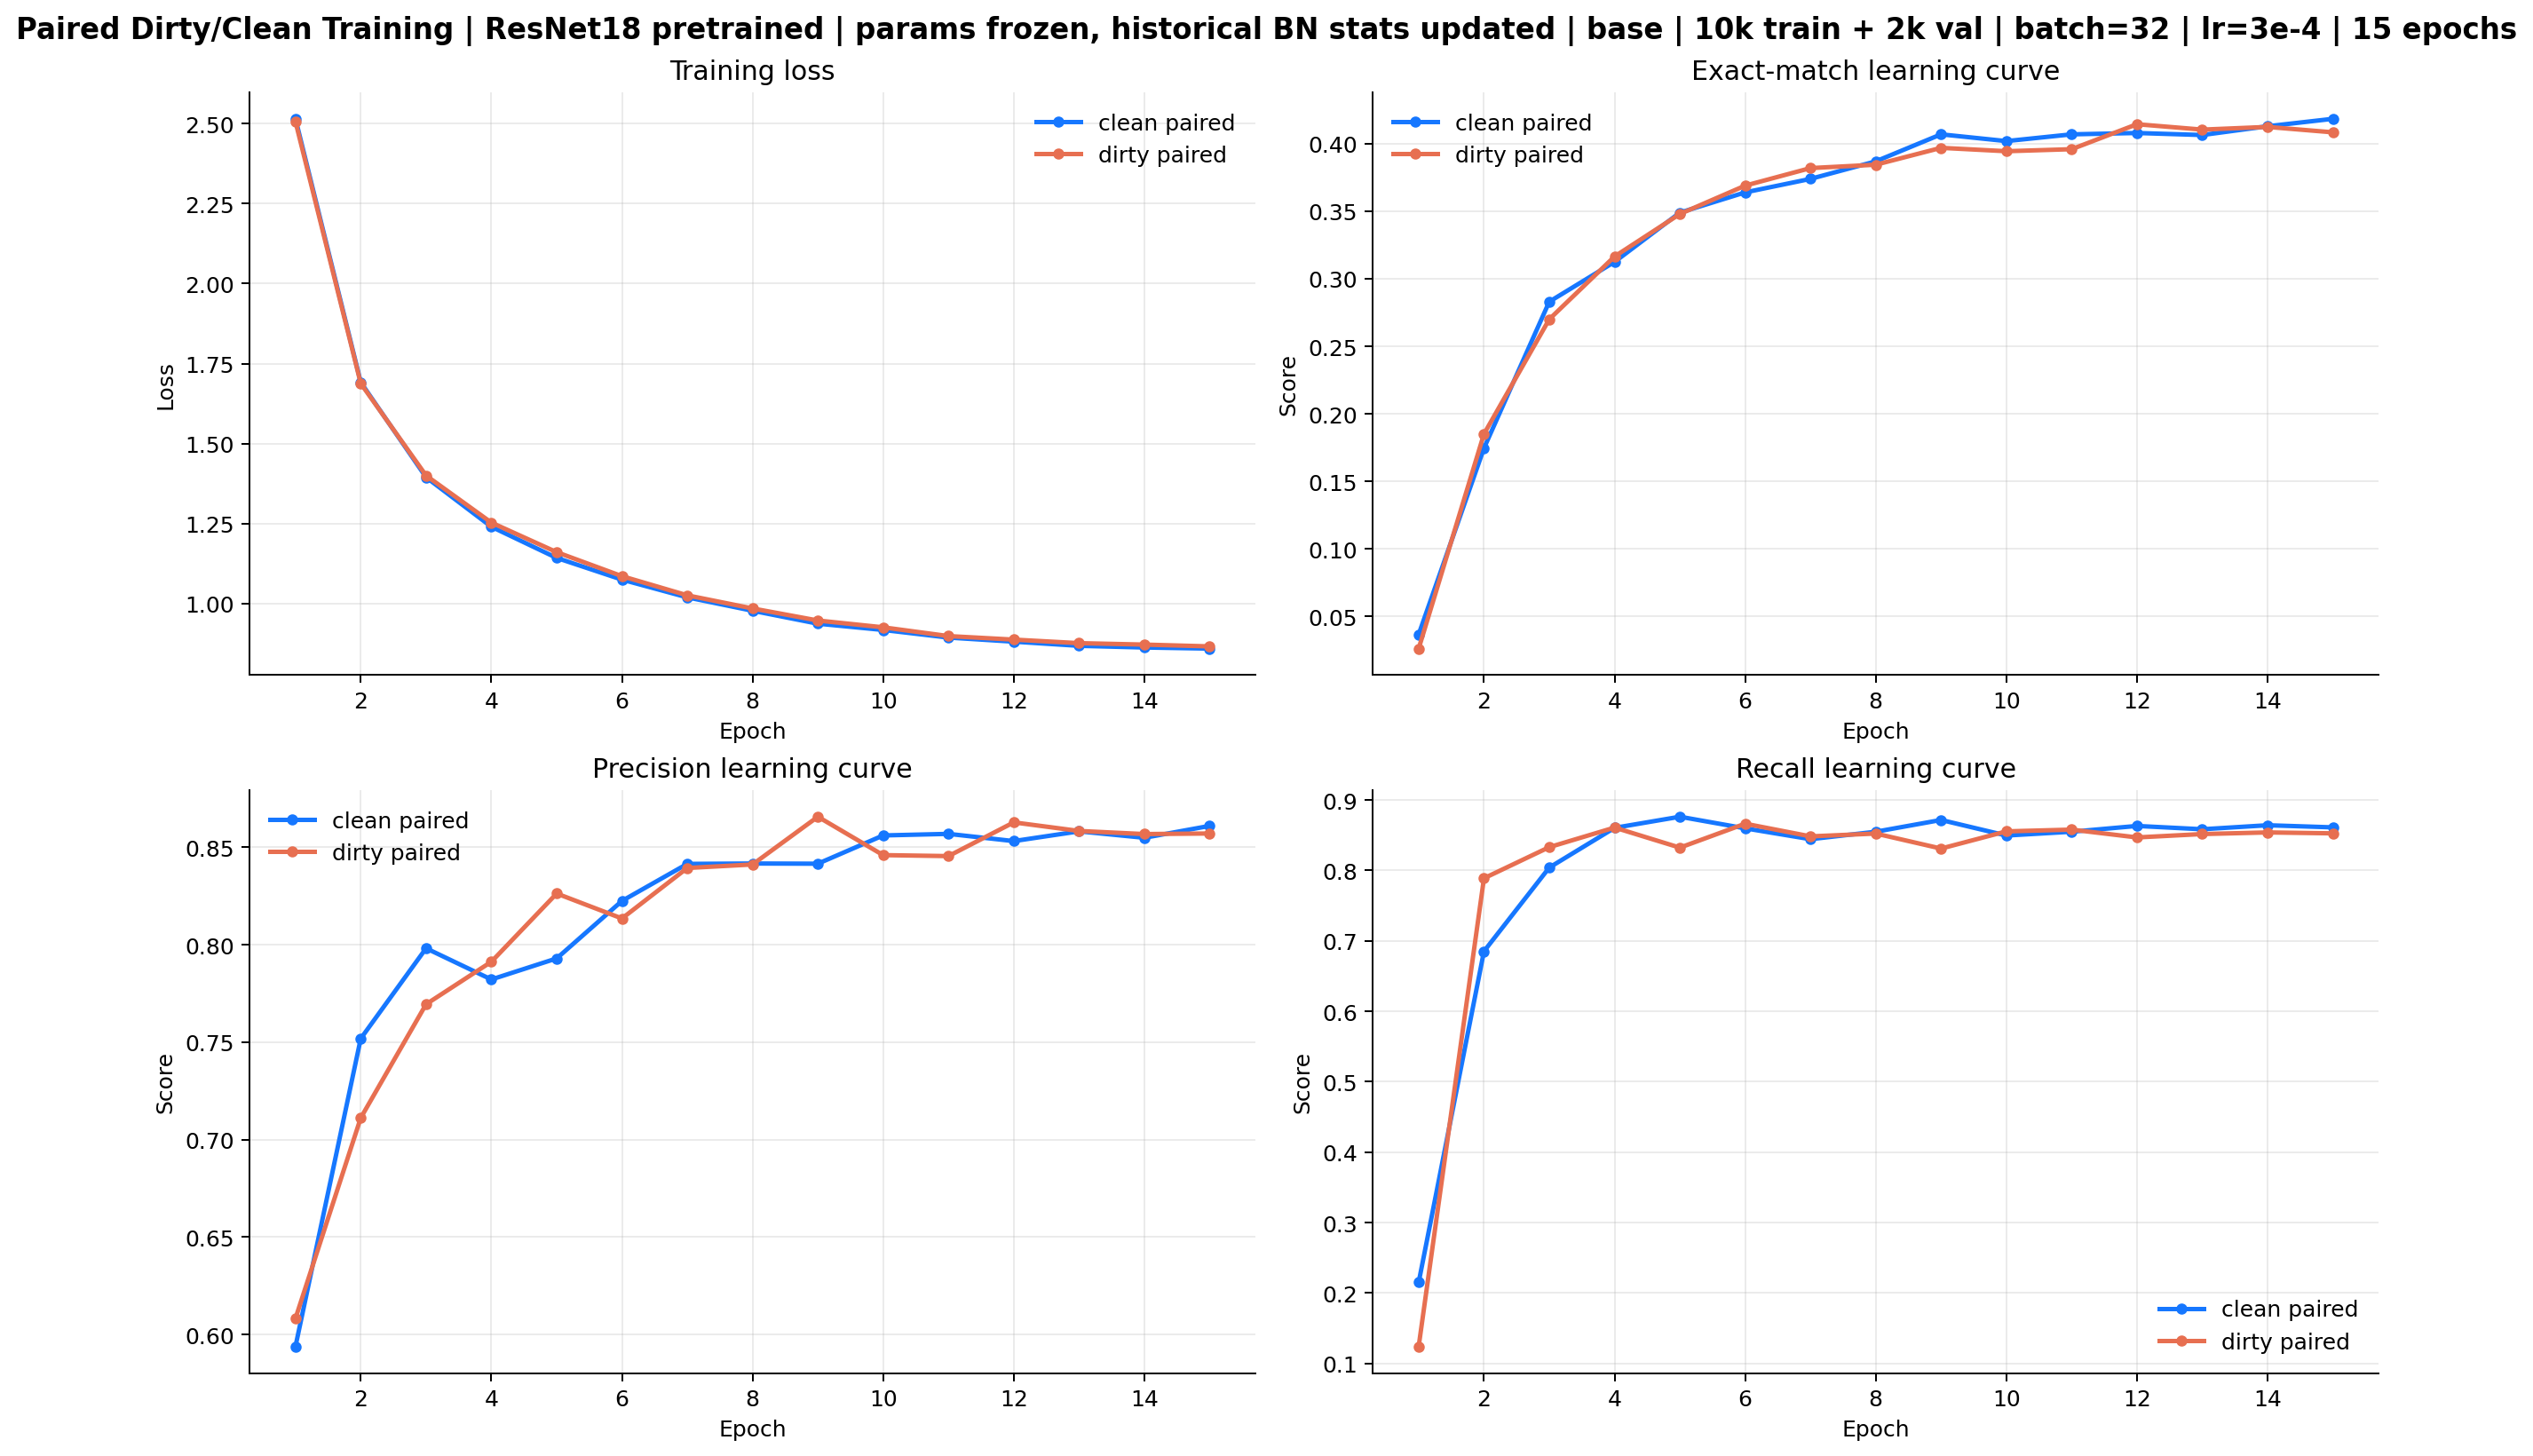
\includegraphics[width=0.96\linewidth]{dirty_clean_training_curves.png}
  \caption{Paired dirty/clean 训练与验证曲线。两组实验的损失与 exact match 收敛过程非常接近，clean paired 在训练后期呈现略高的 exact match 和 recall，与测试集上“改善有限但方向一致”的结果相符。}
  \label{fig:dirty-clean-training-curves}
\end{figure}

这个结果没有表现为“大幅跃升”，但对项目决策很重要：弱类失败并不完全是模型容量问题，源图质量、类别语义边界和阈值策略同样影响最终动作序列。裙子、帐篷、船、人、玩具等类别容易出现目标过小、裁剪不完整、主体不明确或类内差异过大的问题，因此后续应继续采用人工 contact sheet review、per-class blacklist 和固定实验集，而不是只增加训练轮数。

\subsection{专训模型与多模态大模型对比}

为了检验通用多模态大模型能否直接替代本项目专训模型，我们在同一 clean paired 测试集上接入 Qwen3-VL-Flash baseline。评估方式要求模型阅读九宫格图片和中文提示，输出所有应点击格子。表~\ref{tab:vlm-compare} 显示，Qwen3-VL-Flash 的 cell exact match 为 14.75\%，明显低于本项目 ResNet18 action 模型的 46.00\%。这并不说明通用 VLM 视觉能力弱，而是说明在低分辨率九宫格、固定格子编号、多目标数量判断和严格集合匹配的任务协议下，经过同分布数据专训的小模型具有明显优势。

\begin{table}[H]
  \centering
  \caption{同一 clean paired 测试集上的专训模型与多模态大模型对比。}
  \label{tab:vlm-compare}
  \scriptsize
  \begin{tabular}{p{0.30\linewidth}ccccc}
    \toprule
    \rowcolor{tablehead}
    方法 & 测试样本 & Cell Exact $\uparrow$ & Precision $\uparrow$ & Recall $\uparrow$ & Count Acc. $\uparrow$ \\
    \midrule
    RoboTest ResNet18 action（参数冻结，BN 统计量适配） & 2000 & 0.4600 & 0.8677 & 0.8750 & -- \\
    Qwen3-VL-Flash & 2000 & 0.1475 & 0.6998 & 0.6081 & 0.3880 \\
    \bottomrule
  \end{tabular}
\end{table}

\begin{figure}[H]
  \centering
  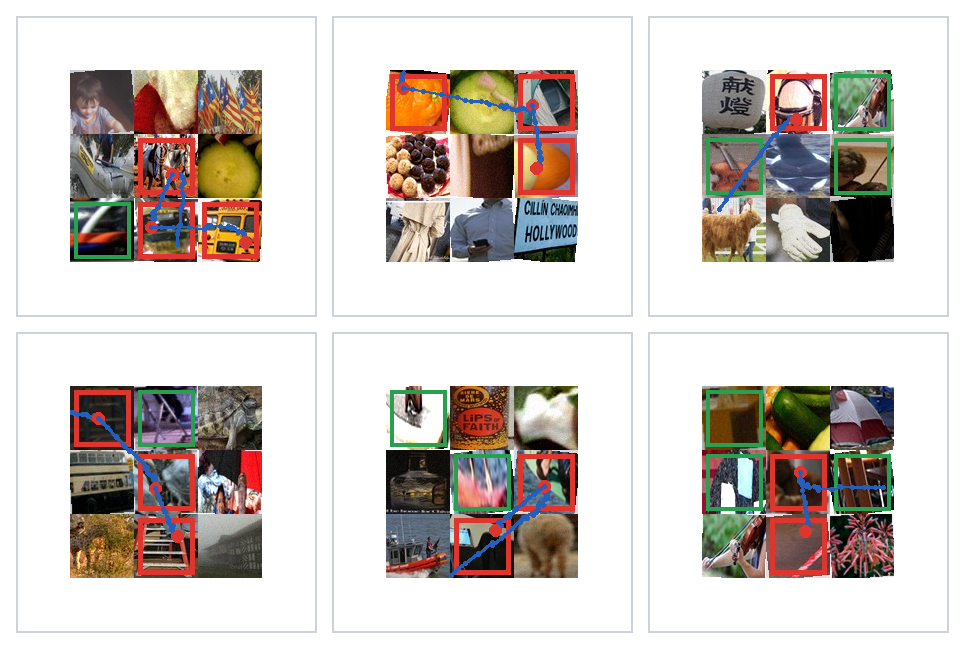
\includegraphics[width=0.84\linewidth]{failure_vlm_montage.png}
  \caption{Qwen3-VL-Flash baseline 的失败样例拼图。通用 VLM 能识别部分目标，但在低分辨率九宫格、严格格子编号和多目标集合输出上容易出现漏点或多点。}
  \label{fig:results-comparison}
\end{figure}

定性观察显示，VLM baseline 经常能识别部分目标，但容易出现三类错误：第一，低分辨率 cell 中的物体细节不足，导致类别判断不稳定；第二，模型需要同时输出多个格子时容易漏点或多点；第三，格子编号协议与自然语言视觉问答习惯不同，需要更强的 prompt engineering 或专门的 GUI grounding 训练。这个对比帮助我们明确了项目价值：通用 VLM 可以作为强基线和演示补充，但在固定任务上仍需要专门数据、专门指标和专门训练。

\section{结果分析}

实验结果首先验证了任务难度设计的合理性。easy 数据中颜色唯一，规则颜色基线即可完成任务；medium 数据中颜色重复，单纯颜色匹配会产生歧义；hard 数据中提示不含颜色，模型必须依赖形状或语义特征。颜色基线从 easy 的 1.000 下降到 hard 的 0.111，说明该难度划分确实能区分不同层次的视觉理解能力。

早期结果偏高的主要原因不是模型已经解决了真实问题，而是任务协议较干净。合成图形中对象形状规则、背景简单、颜色和类别由程序控制，模板图文匹配天然占优；早期真实照片九宫格按样本级划分训练/验证集，同一原始 source 图片可能以不同组合出现在不同 split，导致验证集仍与训练集共享视觉来源。因此，早期 100 类照片 attention 模型的 82.4\% Top-1 和 96.87\% Top-3 更适合说明“模型能利用该照片库学习图文匹配”，但不能直接证明对全新来源图片的严格泛化。

这一发现改变了后续工作重点。我们没有继续把“训练时间不够”当作默认解释，而是先做失败图检查和数据构建器改造。失败样例显示，弱类错误常常来自数据本身：裙子可能只露出局部布料，帐篷和船的视角差异很大，人类类别过宽，玩具类别语义边界不清，部分原图目标面积很小或长宽比极端。于是项目加入 source-disjoint split、source area/aspect ratio 过滤、弱类 blacklist、paired dirty/clean 实验和 per-class metrics。这些改动虽然只带来约 0.95 个百分点的 exact match 提升，但它们让后续实验更可信，因为提升来自可追溯的数据质量控制，而不是不可解释的随机训练波动。

Click-all 任务的难点也不同于单目标分类。单目标任务只需选一个最高分 cell，而 click-all 任务要求同时判断目标集合和目标数量。因此 exact match 对漏点和误点都非常敏感：只要少点一个目标或多点一个干扰 cell，样本就算失败。当前 clean 模型的 exact match 为 46.00\%，但 precision 和 recall 均约为 0.87，说明模型通常能找到大部分正确目标，只是在集合完全一致和点击数量控制上仍不稳定。这也解释了为什么阈值校准比单纯加模型层数更关键。

\begin{figure}[H]
  \centering
  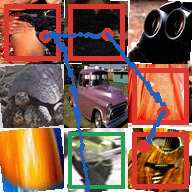
\includegraphics[width=0.62\linewidth]{click_all_failure_example.png}
  \caption{Click-all 失败样例。失败图用于区分漏点、多点、弱类源图质量问题和阈值选择问题，是后续数据清洗的重要依据。}
  \label{fig:click-all-failure}
\end{figure}

与 Qwen3-VL-Flash 的对比进一步说明了任务特性。通用 VLM 具备更强开放世界语义知识，但它没有针对本项目的格子编号、低分辨率 cell、多目标集合输出和严格评估协议训练，因此在 exact match 上明显落后于专训模型。这个结果给我们的启发是：在课程项目或实际工程中，通用大模型可以承担 prompt rewrite、抽象语义解释和备选 baseline，但核心定位模型仍需要围绕具体数据分布和评价指标做专门训练。

综上，当前项目的主要经验是：模型结构、数据质量和评估协议必须一起设计。若只看合成数据准确率，容易过早得出“模型已经很好”的结论；若只看真实数据下降，又容易误判为模型容量不足。更可靠的路线是固定实验集、消除 source 泄露、分析失败类别、清洗数据，再决定是否引入更大的视觉编码器或多模态预训练模型。

\section{算法代码及实现说明}

项目代码按功能模块组织，主要文件如下：

\begin{longtable}{p{0.28\linewidth}p{0.64\linewidth}}
  \caption{主要代码文件及功能说明。}
  \label{tab:code-files}\\
  \toprule
  \rowcolor{tablehead}
  文件 & 功能 \\
  \midrule
  \endfirsthead
  \toprule
  \rowcolor{tablehead}
  文件 & 功能 \\
  \midrule
  \endhead
  \pathcode{src/multimodal_captcha/generator.py} & 生成合成九宫格数据、中文提示、目标标签和多目标动作序列标签。\\
  \pathcode{src/multimodal_captcha/dataset.py} & 读取 manifest 文件，构造 PyTorch Dataset，完成图像加载、文本编码和 train/val 划分。\\
  \pathcode{src/multimodal_captcha/model.py} & {\raggedright 定义 \code{MultimodalGridLocator}、\code{ActionSequenceLocator} 和最终 click-all 模型 \code{ActionCellSelector}，实现 CNN、GRU、Transformer 和图文融合结构。\par}\\
  \pathcode{src/multimodal_captcha/action_sequence.py} & 定义 click-all 任务中 target indices、动作 token 和点击 cell 集合之间的转换逻辑。\\
  \pathcode{src/multimodal_captcha/action_checkpoint.py} & 保存和加载 action sequence checkpoint，记录模型配置、vocab 和 object vocab。\\
  \pathcode{src/multimodal_captcha/query_planner.py} & 将自然语言提示解析为对象、颜色、位置和大小等结构化查询。\\
  \pathcode{src/multimodal_captcha/attribute_scorer.py} & 实现颜色、位置、大小等轻量属性 scorer，补充主模型无法直接处理的提示类型。\\
  \pathcode{src/multimodal_captcha/prompt_rewriter.py} & 接入 DeepSeek API 或规则 fallback，将抽象提示改写为训练类别提示。\\
  \pathcode{src/multimodal_captcha/vlm_baseline.py} & 封装多模态大模型 baseline，用于在自建数据集上和专训模型对比。\\
  \pathcode{src/multimodal_captcha/baseline.py} & 实现规则颜色基线。\\
  \pathcode{src/multimodal_captcha/template_matcher.py} & 实现模板图文匹配模型。\\
  \pathcode{src/multimodal_captcha/trajectory.py} & 根据预测点击点生成平滑鼠标轨迹。\\
  \pathcode{scripts/train.py} & 训练九宫格定位模型，保存 checkpoint 和 JSONL 日志。\\
  \pathcode{scripts/evaluate.py} & 批量评估模型，输出 accuracy、Top-3、点击距离和失败案例。\\
  \pathcode{scripts/build_photo_grid_dataset.py} & 从真实照片类别目录构造九宫格数据集，并支持 hard augmentation。\\
  \pathcode{scripts/build_photo_action_dataset.py} & 构造 click-all 真实照片动作序列数据，支持 source-disjoint split、质量过滤、blacklist 和 paired dirty/clean 实验。\\
  \pathcode{scripts/train_action_sequence.py} & 训练 click-all action sequence 模型，支持 CPU/GPU、ResNet18 encoder、auto config 保存。\\
  \pathcode{scripts/evaluate_action_sequence.py} & 评估 click-all 模型，输出 exact match、precision、recall、阈值搜索结果和失败图。\\
  \pathcode{scripts/evaluate_vlm_action_sequence.py} & 调用 VLM API 在同一 click-all 测试集上输出 baseline 结果。\\
  \pathcode{scripts/predict_action_sequence.py} & 对单张图片执行 click-all 推理，输出 JSON 动作序列和可视化图片。\\
  \pathcode{scripts/make_demo_html.py} & 生成静态 HTML 可视化预测结果。\\
  \pathcode{app.py} & Streamlit 交互式演示页面。\\
  \bottomrule
\end{longtable}

项目的最小复现实验可以通过以下命令完成：

\begin{verbatim}
python scripts/generate_dataset.py --num-samples 600 --difficulty medium
python scripts/train.py --epochs 2 --batch-size 64 \
  --output outputs/model.pt --progress-every 5
python scripts/evaluate.py --mode model --checkpoint outputs/model.pt
streamlit run app.py --server.port 8501
\end{verbatim}

真实照片 100 类模型可使用 \code{brief.md} 中记录的训练命令复现。若不重新训练，也可以直接加载已有 checkpoint 进行单张图片预测：

\begin{verbatim}
python scripts/predict_image.py \
  --image path/to/your_grid.png \
  --prompt "请点击汽车" \
  --checkpoint outputs/photo_model_100cls_attn.pt \
  --output outputs/custom_prediction.png
\end{verbatim}

\section{系统展示方式}

项目提供 Streamlit Web 页面作为最终展示入口，运行命令为：
\begin{verbatim}
streamlit run app.py --server.port 8501
\end{verbatim}

页面主要包含三个展示方向：
\begin{itemize}[leftmargin=2em]
  \item \textbf{单目标 grounding 展示：}用户可以选择或上传九宫格图片，输入中文 prompt，系统显示预测格子、点击点、概率分布和可视化结果；
  \item \textbf{Click-all action sequence 展示：}用户输入“请点击所有汽车”等指令后，系统输出所有预测目标格、对应动作 token、JSON 结果和标注后的图片；
  \item \textbf{提示词与大模型对比展示：}页面可以启用 DeepSeek prompt rewrite、结构化 query planner 和多模态大模型 baseline，与本地专训模型在同一图片上并排对比。
\end{itemize}

展示系统的设计目标是让实验结果可检查、可复现、可解释。用户不需要阅读训练日志，也可以直观看到模型选择了哪些 cell、为什么 click-all 任务会出现漏点或多点、VLM 与专训模型的输出差异在哪里。页面中的官方服务集成仅用于合规展示 CAPTCHA widget 的形式，不把模型用于绕过第三方真实验证码。

\begin{figure}[H]
  \centering
  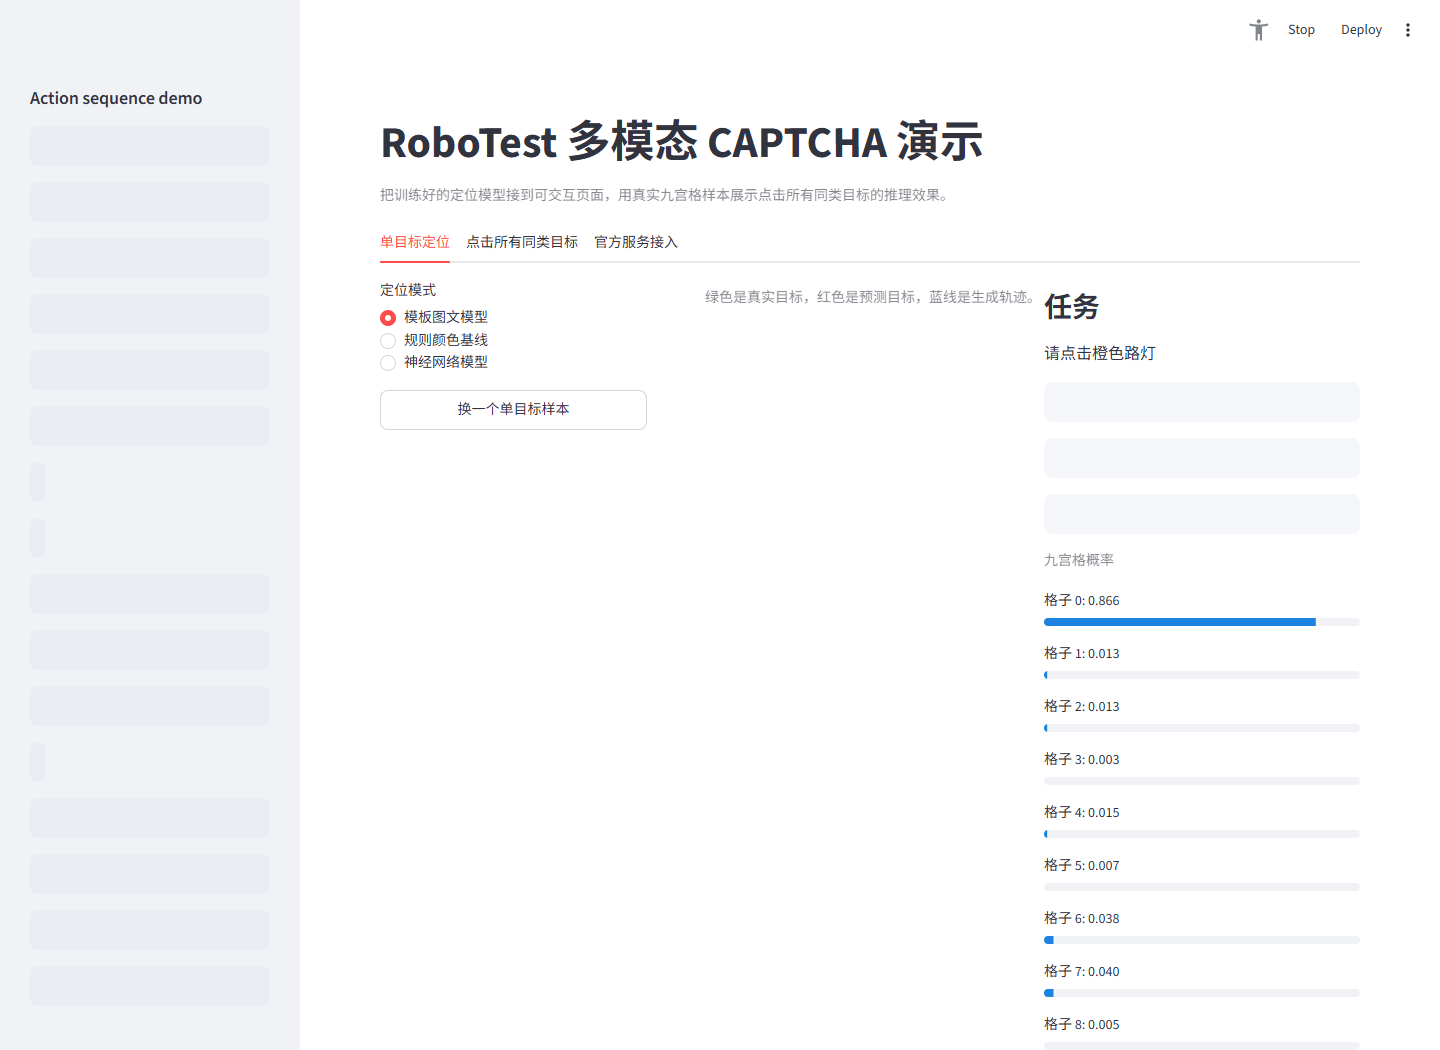
\includegraphics[width=0.96\linewidth]{streamlit_demo.png}
  \caption{Streamlit Web 展示页面截图。页面支持单目标定位、click-all 动作序列、官方服务接入展示、提示词改写和 VLM 对比入口。}
  \label{fig:streamlit-demo}
\end{figure}

\section{创新性}

本项目的创新性主要体现在以下几个方面：
\begin{enumerate}[leftmargin=2em]
  \item \textbf{从普通分类转向九宫格图文 grounding：}项目将中文任务指令、九宫格候选图像和点击动作组织为统一任务，比单图分类更能体现多模态对齐能力；
  \item \textbf{从单目标预测扩展到 click-all 动作序列：}输出从一个格子编号升级为可执行动作 token 序列，更接近连续点击多个目标的真实场景；
  \item \textbf{从随机九宫格升级为相似类别与 source-disjoint 数据：}参考 PPT 中“相似类别九宫格”的设计，迫使模型学习 prompt 与局部图像的细粒度匹配，而不是依赖粗粒度外观；
  \item \textbf{从盲目加模型转向数据质量驱动：}通过 paired dirty/clean、弱类 blacklist、source quality filter 和阈值校准分析性能瓶颈；
  \item \textbf{从封闭类别扩展到自然提示处理：}加入 prompt rewrite、query planner 和属性 scorer，补足颜色、位置、大小、功能性表达等提示类型；
  \item \textbf{从离线实验扩展到 Web 可解释展示：}Streamlit 页面整合本地专训模型、VLM baseline、JSON 动作输出和失败图可视化，方便演示与复盘。
\end{enumerate}

\section{局限性与后续改进}

当前项目仍有若干局限。首先，真实照片数据来源虽然比合成图形复杂，但仍是从公开数据集中裁剪并重新拼接的九宫格，与真实网页验证码中的街景、多尺度目标、遮挡和动态交互仍有差距。其次，虽然 click-all 数据已经采用 source-disjoint split，但早期单目标实验仍存在样本级划分带来的潜在高估，报告中相关结论需要明确限定在对应数据协议内。再次，当前主模型对颜色、空间关系和抽象语义的理解主要依赖规则模块或提示词改写，尚未通过统一模型端到端学习。最后，鼠标轨迹仍由规则生成，并不是从真实人类轨迹数据中学习得到，因此只能作为交互流程模拟，不能代表真实行为验证。

后续改进可以从五个方向推进：
\begin{enumerate}[leftmargin=2em]
  \item \textbf{固定实验集与数据审计：}继续维护 source-disjoint benchmark、contact sheet review、per-class blacklist 和可追溯数据版本；
  \item \textbf{更真实的数据生成：}加入小目标、遮挡、低清晰度、复杂背景、真实网页截图风格和更复杂的候选区域布局；
  \item \textbf{更强但可控的模型：}比较 frozen/fine-tuned ResNet、ViT、CLIP、GUI-specialized VLM 和 cross-attention 模型，区分数据收益与模型收益；
  \item \textbf{更完整的动作任务：}支持“按顺序点击”“点击某物右侧目标”“连续点击多张图片”等多步任务，并把点击顺序纳入训练目标；
  \item \textbf{轨迹/控制代码新模态：}收集或模拟更真实的鼠标轨迹，将 cell selection、click order 和 trajectory realism 分开评估，再尝试 learned trajectory decoder。
\end{enumerate}

\section{项目学习体会}

这个项目最大的收获是，我们对“模型效果好不好”的判断从单一准确率转向了完整实验协议。最开始，合成数据和早期真实照片结果很容易让人觉得任务已经解决；但进一步检查失败图、数据来源和 split 方式后，我们意识到结果可能受到模板规则、数据泄露和源图质量影响。这个过程让我们认识到，在多模态任务中，数据构建和评估协议往往和模型结构同等重要。

第二个收获是，小数据量场景下不能盲目相信更大的模型。ResNet 微调、CLIP zero-shot、Qwen-VL baseline 都提供了有价值的参照，但最终在我们自己的固定九宫格任务上，经过 source-disjoint 数据、阈值校准和任务专训的小模型反而更稳定。这说明工程上应先明确任务分布、指标和错误类型，再决定是否引入更复杂的预训练模型。

第三个收获是，多模态系统不是简单把图像模型和文本模型拼接起来。真实用户提示可能包含颜色、位置、功能、抽象类别和多步动作，例如“红色物体”“可以演奏音乐的物体”“点击所有同类目标”。这些需求要求系统同时具备类别映射、属性解析、视觉定位、动作序列生成和可视化解释能力。RoboTest 当前还只是一个课程原型，但它已经让我们完整经历了从任务定义、数据生成、模型训练、失败分析、基线对比到 Web 展示的闭环。

\section{结论}

本文设计并实现了一个面向多模态数据分析课程的九宫格图文定位与动作序列系统。该系统以中文指令和九宫格图像为输入，通过规则基线、模板匹配、神经网络模型和 VLM baseline 完成目标格预测，并进一步输出点击动作序列和可视化结果。实验表明，简单颜色基线只能解决颜色信息充分的 easy 任务，模板图文匹配能稳定处理合成图形任务，而专训 action 模型在 source-disjoint clean paired click-all 数据集上明显优于直接调用通用 VLM 的 baseline。更重要的是，项目过程表明数据泄露、源图质量、弱类语义边界和阈值策略会显著影响实验结论。未来工作将围绕固定真实实验集、GUI-specialized VLM、属性与关系提示、连续动作序列和鼠标轨迹新模态继续推进。

\clearpage
\appendix

\section{附录：复现实验命令}

\subsection{构造 100 类真实照片九宫格数据}
\begin{verbatim}
python scripts/build_photo_grid_dataset.py \
  --photo-root data/photo_objects \
  --output-dir data/photo_grid_100cls \
  --num-samples 10000 \
  --min-images-per-class 100 \
  --max-classes 120 \
  --hard-augment \
  --progress-every 100
\end{verbatim}

\subsection{训练 attention 模型}
\begin{verbatim}
python scripts/train.py \
  --data-dir data/photo_grid_100cls \
  --output outputs/photo_model_100cls_attn.pt \
  --epochs 40 \
  --batch-size 64 \
  --lr 0.001 \
  --aux-weight 0.7 \
  --patience 10 \
  --model-size attn \
  --progress-every 20
\end{verbatim}

\subsection{评估模型}
\begin{verbatim}
python scripts/evaluate.py \
  --data-dir data/photo_grid_100cls \
  --mode model \
  --checkpoint outputs/photo_model_100cls_attn.pt \
  --output-dir outputs/eval_100cls_attn \
  --progress-every 100
\end{verbatim}

\subsection{生成静态 HTML 可视化}
\begin{verbatim}
python scripts/make_demo_html.py \
  --data-dir data/photo_grid_100cls \
  --mode model \
  --checkpoint outputs/photo_model_100cls_attn.pt \
  --output outputs/photo_demo_100cls_model.html \
  --num-examples 12
\end{verbatim}

\subsection{构造 click-all paired 数据集}
\begin{verbatim}
python scripts/build_photo_action_dataset.py \
  --photo-root data/photo_objects \
  --output-dir data/photo_action_click_all_clean80_paired_10k \
  --source-pool-manifest outputs/paired80_source_pool.json \
  --source-split-plan outputs/paired80_source_split_plan.json \
  --bad-source-labels outputs/failure_analysis/bad_source_labels.json \
  --missing-plan-source-policy skip \
  --num-train 10000 \
  --num-val 2000 \
  --num-test 2000 \
  --image-size 192 \
  --min-targets 2 \
  --max-targets 4 \
  --hard-augment \
  --balanced-targets
\end{verbatim}

\subsection{训练与评估 click-all action 模型}
\begin{verbatim}
python scripts/train_action_sequence.py \
  --data-dir data/photo_action_click_all_clean80_paired_10k \
  --output outputs/action_resnet18_frozen_clean80.pt \
  --image-encoder resnet18 \
  --freeze-image-encoder \
  --epochs 20 \
  --batch-size 32 \
  --device auto \
  --progress-every 20

python scripts/evaluate_action_sequence.py \
  --data-dir data/photo_action_click_all_clean80_paired_10k \
  --checkpoint outputs/action_resnet18_frozen_clean80.pt \
  --split test \
  --threshold auto \
  --output-dir outputs/action_resnet18_frozen_clean80_eval \
  --device auto
\end{verbatim}

\subsection{评估多模态大模型 baseline}
\begin{verbatim}
python scripts/evaluate_vlm_action_sequence.py \
  --data-dir data/photo_action_click_all_clean80_paired_10k \
  --split test \
  --provider qwen \
  --model qwen3-vl-flash \
  --output-dir outputs/vlm_action_eval_qwen \
  --resume \
  --progress-every 20
\end{verbatim}

\subsection{启动 Web 展示}
\begin{verbatim}
streamlit run app.py
\end{verbatim}

\clearpage
\section{附录：核心算法代码}

本附录摘录实验中直接决定模型输出的核心实现。代码由 \code{listings} 从仓库源文件直接引用，行号与当前提交版本一致；数据加载、命令行解析和 Web 展示等工程性代码未重复附上，完整实现见项目仓库。

\subsection{九宫格图文特征融合}

\pathcode{src/multimodal_captcha/model.py} 中的 \code{MultimodalGridLocator} 使用双向 GRU 编码中文指令，将整张图像切分为九个 cell，通过共享视觉编码器提取特征。下面的构造代码定义了特征投影、位置编码、Transformer 上下文建模和交互融合层。

\lstinputlisting[
  style=robotestpython,
  firstline=133,
  lastline=174,
  firstnumber=133,
  caption={文本、图像与九格上下文模块。},
  label={lst:grid-locator-init}
]{../src/multimodal_captcha/model.py}

前向计算先对九个 cell 统一 resize 并编码，再将 cell 特征与文本特征、逐元素乘积和绝对差拼接，最终为每个格子输出一个定位 logit。

\lstinputlisting[
  style=robotestpython,
  firstline=182,
  lastline=218,
  firstnumber=182,
  caption={九宫格切分、编码与图文融合前向计算。},
  label={lst:grid-locator-forward}
]{../src/multimodal_captcha/model.py}

\subsection{Click-all 多目标格子选择}

\code{ActionCellSelector} 复用上述图文编码器，但不再对九个格子做单标签 softmax，而是独立输出每格 logit。可选的 count head 同时预测点击数量，用于 top-k 解码。

\lstinputlisting[
  style=robotestpython,
  firstline=258,
  lastline=326,
  firstnumber=258,
  caption={Click-all cell selector 与目标数量辅助头。},
  label={lst:action-cell-selector}
]{../src/multimodal_captcha/model.py}

\subsection{动作序列编码与解码}

动作序列模块将目标格集合转换为 \code{move\_to\_cell}、\code{click} 和 \code{done} 序列，并在动作字典与 JSON 形式之间双向转换。完整实现位于 \pathcode{src/multimodal_captcha/action_sequence.py}。

\lstinputlisting[
  style=robotestpython,
  firstline=8,
  lastline=63,
  firstnumber=8,
  caption={动作 token 定义及动作序列双向转换。},
  label={lst:action-token-codec}
]{../src/multimodal_captcha/action_sequence.py}

推理阶段支持两种解码方式：阈值解码根据每格 sigmoid 概率选择所有目标，若没有格子超过阈值则回退到 argmax；top-k 解码先由 count head 预测数量，再选取得分最高的 $k$ 个格子。

\lstinputlisting[
  style=robotestpython,
  firstline=124,
  lastline=148,
  firstnumber=124,
  caption={基于阈值和预测数量的 click-all 解码。},
  label={lst:action-decode}
]{../src/multimodal_captcha/action_sequence.py}

\subsection{鼠标轨迹生成}

\pathcode{src/multimodal_captcha/trajectory.py} 在预测格内随机选择落点，并依据起点到落点的距离自适应确定步数。轨迹通过 easing、法向弯曲、中段抖动、随机停顿和终点微抖动组合生成。

\lstinputlisting[
  style=robotestpython,
  firstline=21,
  lastline=67,
  firstnumber=21,
  caption={格内落点与平滑鼠标轨迹生成。},
  label={lst:mouse-trajectory}
]{../src/multimodal_captcha/trajectory.py}

\end{document}
